% #############################################################################
% This is the MAIN DOCUMENT of the Thesis MSc TEMPLATE.
% The content for the Thesis MSc is to be written in separate documents
% located in the folder ./Chapters
%         Aknowledgments.tex
%         Abstract.tex
%         KeyWords.tex
%         Resumo.tex
%         PalavrasChave.tex
%         Acronyms.tex
%         Front_Cover.tex
%         Chapter_1.tex ....Chapter_2 .....
%         ApendixA.tex ... ApendixB.tex...
% -----------------------------------------------------------------------------
% The class "istulthesis" is based on the standard LaTeX 'report' class.
% It can be used for Instituto Superior Tecnico thesis, as it follows the 
% regulations published by the Scientific Council of IST.
% The class defines the document style. 
% IST requires the thesis to be written in Arial or similar. 
% Two arguments in '\documentclass' allow you to define the thesis font: 
% 'Helvetica' and 'AvantGarde', which transforms 
% the default LaTeX font into Helvetica or AvantGarde, respectively.
% #############################################################################
% The document is automatically set for english or portuguese by just selecting
% the MAIN LANGUAGE in file 'Thesis-MSc-Preamble_commands.tex' 
% #############################################################################
% Thesis-MSc
% Version 2.0, August 2018
% BY: Rui Santos Cruz, rui.s.cruz@tecnico.ulisboa.pt
% #############################################################################
% !TEX root = ./main.tex
% -----------------------------------------------------------------------------
%
\documentclass[defaultstyle,10pt,Helvetica]{istulthesis}
%
% -----------------------------------------------------------------------------
% The Preamble document contains all the necessary Packages for typesetting
% Modify it to suit your needs
% -----------------------------------------------------------------------------
% #############################################################################
% Preamble for Thesis-MSc in English or Portuguese
% Required Packages and commands
% --> Please Choose the MAIN LANGUAGE for the Thesis in package BABEL (below)
% !TEX root = ./main.tex
% #############################################################################
% Thesis-MSc
% Version 2.0, August 2018
% BY: Rui Santos Cruz, rui.s.cruz@tecnico.ulisboa.pt
% #############################################################################
%
% -----------------------------------------------------------------------------
% PACKAGES ucs, utf8x, babel, iflang:
% -----------------------------------------------------------------------------
\usepackage[utf8]{inputenc}
% The 'ucs' package provides support for using UTF-8 in LaTeX documents. 
% However in most situations it is not required.
%\usepackage{ucs}
% The 'utf8x' package contains support for using UTF-8 as input encoding. 
%\usepackage[utf8x]{inputenc}
% The 'babel' package may correct some hyphenation issues of LaTeX. 
% Select your MAIN LANGUAGE for the Thesis with the 'main=' option.
\usepackage[main=english,portuguese]{babel}
% The 'iflang' package is used to help determine the language being used. 
\usepackage{iflang}

% -----------------------------------------------------------------------------
% PACKAGE biblatex:
% -----------------------------------------------------------------------------
\usepackage[backend=biber]{biblatex}


% -----------------------------------------------------------------------------
% PACKAGE scrbase:
% -----------------------------------------------------------------------------
% The 'scrbase' package is used to help redefining document structure.
\usepackage{scrbase}
% -----------------------------------------------------------------------------
% PACKAGE mathtools, amsmath, amsthm, amssymb, amsfonts, nicefrac:
% -----------------------------------------------------------------------------
% These packages are typically required. 
% Among many other things they add the possibility to put symbols in bold
% by using \boldsymbol (not \mathbf); defines additional fonts and symbols;
% adds the \eqref command for citing equations.
\usepackage{mathtools, amsmath, amsthm, amssymb, amsfonts}
\usepackage{nicefrac}
%
% -----------------------------------------------------------------------------
% PACKAGE tikz:
% -----------------------------------------------------------------------------
% Tikz  for creating graphics programmatically.
\usepackage{tikz}
\usetikzlibrary{shapes.geometric, arrows, positioning}
% -----------------------------------------------------------------------------
% PACKAGES array, booktabs, multirow, colortbl, ctable, spreadtab:
% -----------------------------------------------------------------------------
% These packages are most usefull for advanced tables. 
% 'multirow' allows to join rows throuhg the command \multirow which works
% similarly with the command \multicolumn.
% The 'colortbl' package allows to color the table (foreground and background)
% The 'ctable' package provides commands to easily typeset centered or left or
% right aligned tables.
% The package 'booktabs' provide some additional commands to enhance
% the quality of tables
% The 'longtable' package is only required when tables extend beyond the length
% of one page, which typically does not happen and should be avoided
\usepackage{array}
\usepackage{booktabs}
\usepackage{multirow}
\usepackage{colortbl}
\usepackage{ctable}
\usepackage{spreadtab}
\usepackage{longtable}
%
% -----------------------------------------------------------------------------
% PACKAGES graphicx, subfigure:
% -----------------------------------------------------------------------------
% The package 'graphicx' supports formats PNG and JPG.
% Package 'subfigure' allows to place figures within figures with own caption. 
% For each of the subfigures use the command \subfigure.
\usepackage{graphicx}
\usepackage[hang,small,bf,tight]{subfigure}
%
% -----------------------------------------------------------------------------
% PACKAGE caption:
% -----------------------------------------------------------------------------
% The 'caption' package offers customization of captions in floating 
% environments such figure and table
% \usepackage[hang,small,bf]{caption}
\usepackage[format=hang,labelfont=bf,font=small]{caption} 
% the following customization adds vertical space between caption and the table
\captionsetup[table]{skip=10pt}
%
% -----------------------------------------------------------------------------
% PACKAGE algorithmic, algorithm, algorithm2e:
% -----------------------------------------------------------------------------
% These packages are required if you need to describe an algorithm.
% The preference is for using 'algorithm2e'
%\usepackage{algorithmic}
%\usepackage[chapter]{algorithm}
\usepackage[ruled,vlined,algochapter,norelsize,\languagename]{algorithm2e}
%
% -----------------------------------------------------------------------------
% PACKAGE listings
% -----------------------------------------------------------------------------
% These packages are required if you need to list code snippets.
\usepackage{listings}
% Nicely syntax highlighted m-code in LaTeX documents with stylefile mcode.sty
% http://www.mathworks.com/matlabcentral/fileexchange/8015-m-code-latex-package
\usepackage[numbered]{./tables_and_code/mcode}
%
% -----------------------------------------------------------------------------
% Re-define listings captions and titles based on language.
\newcaptionname{portuguese}{\lstlistingname}{Listagem} % Listings CAPTIONS
\newcaptionname{portuguese}{\lstlistlistingname}{Listagens} % LIST of LISTINGS
%
% -----------------------------------------------------------------------------
% PACKAGE csquotes
% -----------------------------------------------------------------------------
% Quotation helper package
\usepackage{csquotes}
%
% -----------------------------------------------------------------------------
% PACKAGE todonotes
% -----------------------------------------------------------------------------
% Create TODO Notes in text
% The notes can be made invisible by just using the 'disable' option:
\usepackage[textwidth=2cm, textsize=small]{todonotes}
%\usepackage[textwidth=2cm, textsize=small, disable]{todonotes}
\setlength{\marginparwidth}{2cm}
%
% -----------------------------------------------------------------------------
% PACKAGE changes
% -----------------------------------------------------------------------------
% Track changes in document (changes in pdf preview).
%% Use "final" option to make all tracking markups invisible.
%\usepackage[authormarkup=superscript,authormarkuptext=id,markup=underlined,ulem={ULforem,normalbf},final]{changes}
\usepackage[authormarkup=superscript,authormarkuptext=id,markup=underlined,ulem={ULforem,normalbf}]{changes}
% commands:
% \added[id=xx]{text}
% \deleted[id=xx]{text}
% \replaced[id=xx]{deleted text}{added text}
% -----------------------------------------------------------------------------
% PACKAGES xcolor, color
% -----------------------------------------------------------------------------
% These packages are required for list code snippets.
\usepackage{xcolor}
\usepackage{color}
% The following special color definitions are used in the IST Thesis
\definecolor{forestgreen}{RGB}{34,139,34}
\definecolor{orangered}{RGB}{239,134,64}
\definecolor{lightred}{rgb}{1,0.4,0.5}
\definecolor{orange}{rgb}{1,0.45,0.13}	
\definecolor{darkblue}{rgb}{0.0,0.0,0.6}
\definecolor{lightblue}{rgb}{0.1,0.57,0.7}
\definecolor{gray}{rgb}{0.4,0.4,0.4}
\definecolor{lightgray}{rgb}{0.95, 0.95, 0.95}
\definecolor{darkgray}{rgb}{0.4, 0.4, 0.4}
\definecolor{editorGray}{rgb}{0.95, 0.95, 0.95}
\definecolor{editorOcher}{rgb}{1, 0.5, 0} % #FF7F00 -> rgb(239, 169, 0)
\definecolor{chaptergrey}{rgb}{0.6,0.6,0.6}
\definecolor{editorGreen}{rgb}{0, 0.5, 0} % #007C00 -> rgb(0, 124, 0)
\definecolor{olive}{rgb}{0.17,0.59,0.20}
\definecolor{brown}{rgb}{0.69,0.31,0.31}
\definecolor{purple}{rgb}{0.38,0.18,0.81}
%
% -----------------------------------------------------------------------------
% PACKAGE setspace:
% ----------------------------------------------------------------------------
% Provides support for setting the spacing between lines in a document. 
% Package options include single spacing, one half spacing, and double spacing. 
% Alternatively the spacing can be changed as required with:
% \singlespacing, \onehalfspacing, and \doublespacing commands
\usepackage{setspace}
%
% -----------------------------------------------------------------------------
% PACKAGE paralist
% -----------------------------------------------------------------------------
% This package provides the 'inparaenum' environment for inline lists
\usepackage{paralist}
% usage:
% \begin{inparaenum}[(a)]
% \item bla
% \item bla, bla
% \end{inparaenum}
% -----------------------------------------------------------------------------
% PACKAGE cite:
% -----------------------------------------------------------------------------
% The 'cite' package will result in citation numbers being automatically
% sorted and properly "ranged". i.e.,
% [1], [2], [5]--[7], [9]
%\usepackage{cite}
%
% -----------------------------------------------------------------------------
% PACKAGE acronym:
% -----------------------------------------------------------------------------
% The package 'acronym' garantees that all acronyms definitions are 
% given at the first usage. 
% IMPORTANT: do not use acronyms in titles/captions; otherwise the definition 
% will appear on the table of contents.
\usepackage[printonlyused]{acronym}
%
% -----------------------------------------------------------------------------
% PACKAGE hyperref
% -----------------------------------------------------------------------------
% Set links for references and citations in document
\usepackage{hyperref}
% pre-configuration of hyperref
\hypersetup{ colorlinks=true,
             citecolor=cyan,
             linkcolor=darkgray,
             urlcolor=teal,
             breaklinks=true,
             bookmarksnumbered=true,
             bookmarksopen=true,
             pdftitle=\@title, % THESIS TITLE
             pdfauthor=\@author,  % YOUR NAME
             pdfcreator=\@author,   % YOUR NAME
}
%
% -----------------------------------------------------------------------------
% PACKAGE url:
% -----------------------------------------------------------------------------
% Provides better support for handling and breaking URLs.
\usepackage{url} 
%
% -----------------------------------------------------------------------------
% PACKAGE Cleveref:
% -----------------------------------------------------------------------------
% Clever Referencing of document parts
% Note: portuguese is supported through "brazilian" option
\usepackage[\IfLanguageName{english}{english}{brazilian}]{cleveref}
%
% -----------------------------------------------------------------------------
% PACKAGE enumitem:
% -----------------------------------------------------------------------------
%For enhanced enumeration of lists
%\usepackage{enumitem}
\usepackage[shortlabels]{enumitem}
\setlist[description]{leftmargin=\parindent,labelindent=\parindent,itemsep=1pt,parsep=0pt,topsep=0pt}
%
% #############################################################################
% GLOBAL FORMATTING OF THE THESIS DOCUMENT before using FANCY stuff
% Set paragraph counter to alphanumeric mode
\renewcommand{\theparagraph}{\Alph{paragraph}~--}
\hoffset 0in
\voffset 0in
\oddsidemargin 0 cm
\evensidemargin 0 cm
\marginparsep 0in
\topmargin -0.25cm
\textwidth 16 cm
\textheight 22.4 cm
\makeatletter
% package indentfirst says \let\@afterindentfalse\@afterindenttrue
% and we revert this modification, reinstating the original definitio
% of \@afterindentfalse
\def\@afterindentfalse{\let\if@afterindent\iffalse}
\makeatother
% -----------------------------------------------------------------------------
% PACKAGE fancyhdr:
% -----------------------------------------------------------------------------
% The fancyhdr macro package allows to customize page headers and footers.
\usepackage{fancyhdr}
\pagestyle{fancy}
\renewcommand{\chaptermark}[1]{\markboth{\thechapter.\ #1}{}}
\renewcommand{\sectionmark}[1]{\markright{\thesection\ #1}}
\fancyhead{}
\renewcommand{\headrulewidth}{0.0pt}
\renewcommand{\footrulewidth}{0.0pt}
\addtolength{\headheight}{2pt} % make space for the rule
\fancypagestyle{plain}{%
   \fancyhead{} % get rid of headers
   \renewcommand{\headrulewidth}{0pt} % and the line
   \renewcommand{\footrulewidth}{0pt}
}
\fancypagestyle{blank}{%
   \fancyhf{} % get rid of headers and footers
   \renewcommand{\headrulewidth}{0pt} % and the line
   \renewcommand{\footrulewidth}{0pt}
}
\fancypagestyle{abstract}{%
   \fancyhead{}
   \renewcommand{\headrulewidth}{0pt}
   \renewcommand{\footrulewidth}{0.0pt}
}
\fancypagestyle{document}{%
	\fancyhead{}
	\renewcommand{\headrulewidth}{0.5pt}
	\renewcommand{\footrulewidth}{0.5pt}
	\addtolength{\headheight}{2pt} % make space for the rule
}
\setcounter{secnumdepth} {5}
\setcounter{tocdepth} {5}
\renewcommand{\thesubsubsection}{\thesubsection.\Alph{subsubsection}}
\renewcommand{\subfigtopskip}{0.3 cm}
\renewcommand{\subfigbottomskip}{0.2 cm}
\renewcommand{\subfigcapskip}{0.3 cm}
\renewcommand{\subfigcapmargin}{0.2 cm}
%
% -----------------------------------------------------------------------------
% PACKAGE minitoc:
% -----------------------------------------------------------------------------
% Package 'minitoc' creates a mini-table of contents (a “minitoc”) at 
% the beginning of each chapter of a document.
% This packages are required for the \fancychapter configuration
\usepackage{minitoc}
\setcounter{minitocdepth}{1}
\setlength{\mtcindent}{24pt}
\renewcommand{\mtcfont}{\small\rm}
\renewcommand{\mtcSfont}{\small\bf}
\renewcommand*{\kernafterminitoc}{\kern0.\baselineskip\kern0.ex}
\mtcselectlanguage{\languagename} 
% Now prepare the MINITOC
\def\boxedverbatim{%
  \def\verbatim@processline{%
    {\setbox0=\hbox{\the\verbatim@line}%
    \hsize=\wd0 \the\verbatim@line\par}}%
  \@minipagetrue%%%DPC%%%
  \@tempswatrue%%%DPC%%%
  \setbox0=\vbox\bgroup\vspace*{0.2cm}\footnotesize\verbatim
}
\def\endboxedverbatim{%
  \endverbatim%
  \unskip\setbox0=\lastbox %%%DPC%%%
  \hspace*{0.2cm}
  \vspace*{-0.2cm}
  \egroup
  \fbox{\box0}% <<<=== change here for centering,...
}
% Now prepare the CHAPTER Number
\newcommand*{\chapnumfont}{%
%   \usefont{T1}{\@defaultcnfont}{b}{n}\fontsize{100}{130}\selectfont%
  \usefont{T1}{pbk}{b}{n}
  \fontsize{150}{130}
  \selectfont
  \color{chaptergrey}
}
\makeatletter
\def\@makechapterhead#1{%
  \vspace*{50\p@}%
  {\parindent \z@ \raggedright \normalfont
    {\chapnumfont\ifnum \c@secnumdepth >\m@ne
%         \huge\bfseries \@chapapp\space \thechapter
        \raggedleft\bfseries \thechapter
        \par\nobreak
        \vskip 20\p@
    \fi}
    \interlinepenalty\@M
    {\raggedleft\Huge \bfseries #1\par\nobreak}
    \vskip 40\p@
  }}
\makeatother
% Now put it all together as a command \fancychapter
\newcommand{\fancychapter}[1]{\chapter{#1}\vfill\minitoc\pagebreak}
%
% #############################################################################
% ADDITIONAL COMMANDS AND CONFIGURATIONS
% #############################################################################
% This commmand allows to place horizontal lines with a custom width... 
% replaces the standard hline command
\newcommand{\hlinew}[1]{%
  \noalign{\ifnum0=`}\fi\hrule \@height #1 \futurelet
   \reserved@a\@xhline}
%   
% -----------------------------------------------------------------------------
% This command defines some marks... USEFUL FOR TABLES.
\def\Mark#1{\raisebox{0pt}[0pt][0pt]{\textsuperscript{\footnotesize\ensuremath{\ifcase#1\or *\or \dagger\or \ddagger\or%
    \mathsection\or \mathparagraph\or \|\or **\or \dagger\dagger%
    \or \ddagger\ddagger \else\textsuperscript{\expandafter\romannumeral#1}\fi}}}}

%
\addbibresource{Thesis-MSc-Bibliography.bib}
% #############################################################################
% #############################################################################
\begin{document}
%
% Add PDF bookmark 
\pdfbookmark[0]{Titlepage}{Title}
% #############################################################################
% DEFINE THE Front Cover Page of Thesis-MSc
% !TEX root = ./main.tex
% #############################################################################
% Thesis-MSc
% Version 2.0, August 2018
% BY: Rui Santos Cruz, rui.s.cruz@tecnico.ulisboa.pt
% #############################################################################
%
% REQUIRED LOGO:
% The university logo image: arguments correspond to {left}{top} position. 
% IST rules determine the position to be be 2cm from top, left page edge
\univlogo{2cm}{2cm}{./Images/IST_A_RGB_POS}
% OPTIONAL IMAGE:
% The thesis image: arguments are the start position in the page.
% You can change the image for your thesis, replacing the image name:
%\thesislogo{2.5cm}{6cm}{./Images/thesis_logo}
\thesislogo{2.5cm}{6cm}{./Images/tecnico-lisboa}
%
% -----------------------------------------------------------------------------
% REQUIRED: Thesis TITLE
\title{Motion Planning for Cooperative Autonomous Robots using optimization Tools}
% OPTIONAL: Thesis SUBTITLE
%\subtitle{This is the Thesis Subtitle if Necessary}
%
% -----------------------------------------------------------------------------
% REQUIRED: Author
% Author full Name
\author{Thomas David Pamplona Berry}
%
% -----------------------------------------------------------------------------
% The official name of the course/degree. Please chose portuguese or english
% un-comment the line corresponding to your degree.
% You can add a degree name using this construct
%
\degree{Electrical and Computer Engineering}
%
% -----------------------------------------------------------------------------
% REQUIRED: The SUPERVISOR(s) - maximum of two
\supervisor{Prof. António Manuel dos Santos Pascoal}
%
% -----------------------------------------------------------------------------
% REQUIRED: Date of examination
% Insert the Date of the Thesis discussion (format is MONTH and YEAR)
\date{December 2020}
%
% -----------------------------------------------------------------------------
% The following command define the author colors for Tracking Changes in doc
\definechangesauthor[color=forestgreen]{MN}
\definechangesauthor[color=blue]{JO}
\definechangesauthor[color=red]{PT}

% -----------------------------------------------------------------------------
% Place 'false' when delivering the draft version of the thesis.
% The committee members should not be printed for the draft version. 
% Place 'true' after the Examination Committee has accepted the thesis as final
%\finalthesis{true}
\finalthesis{true}
%
% -----------------------------------------------------------------------------
% The members of the Examination Committee
\chairperson{Prof. João Fernando Cardoso Silva Sequeira}
\vogalone{Prof. Fernando Lobo Pereira}
%\vogaltwo{Dr. Name of Second Committee Member}
%\vogalthree{Eng. Name of Third Committee Member}
%
% -----------------------------------------------------------------------------
% Please DO NOT MODIFY the following lines.
% print the titlepage
\maketitle
\clearpage
\thispagestyle{empty}

\cleardoublepage
%
% -----------------------------------------------------------------------------
% PAGE NUMBERING FOR INDEXING MATTER in ROMAN
\setcounter{page}{1} \pagenumbering{roman}
\baselineskip 18pt % line spacing: -12pt for single spacing
                   %               -18pt for 1 1/2 spacing
                   %               -24pt for double spacing
% -----------------------------------------------------------------------------
% THE ACKNOWLEGMENTS
\pdfbookmark[0]{Acknowledgments}{acknowledgments}
\begin{acknowledgments}
	% #############################################################################
% Agradecimentos / Acknowledgments
% !TEX root = ../main.tex
% #############################################################################

I would like to thank my parents for their friendship, encouragement and caring over all these years, for always being there for me through thick and thin and without whom this project would not be possible. I would also like to thank my grandparents, aunts, uncles and cousins for their understanding and support throughout all these years.

I would also like to acknowledge my dissertation supervisors Prof. Some Name and Prof. Some Other Name for their insight, support and sharing of knowledge that has made this Thesis possible.

Last but not least, to all my friends and colleagues that helped me grow as a person and were always there for me during the good and bad times in my life. Thank you.

To each and every one of you -- Thank you.
\end{acknowledgments}
%
% -----------------------------------------------------------------------------
% THE ABSTRACT
\pdfbookmark[0]{Abstract}{Abstract}
\begin{abstract}
	\noindent

\par Worldwide, there has been growing interest in the execution of missions of increasing complexity involving the use of several autonomous vehicles acting cooperatively without constant supervision of human operators. A key enabling factor for the execution of such missions is the availability of advanced methods for cooperative motion planning that take explicitly into account temporal and spatial constraints, intrinsic vehicle limitations and energy minimization requirements.
\par Motivated by the current trends in this area of research, the motion planning techniques studied here are tasked with finding feasible and safe trajectories for a group of vehicles such that they reach a number of target points at the same time (the so-called "simultaneous arrival problem") and avoid inter-vehicle as well as vehicle/obstacle collisions, subject to the constraint that the overall energy required for vehicle motion is minimized.
Here, the motion planning problem is formulated as a continuous-time optimal control problem. Different numerical Direct Methods that approximate its solutions in a discretized setting are explored with a focus on Bernstein polynomials. These polynomials possess convenient properties that allow for efficient computation and enforcement of constraints along the vehicles’ trajectories, such as maximum speed, angular rates, and the minimum distance between trajectories along with the minimum distance between the vehicles and known obstacles.
\par Different mathematical tools to calculate cost and feasibility are evaluated. Finally, the results of simulations aimed at showing the efficacy of the complete motion planning algorithm developed for specific numbers of vehicles and different constraints are presented.
\end{abstract}
\begin{keywords}
	% #############################################################################
% English Keywords
% !TEX root = ../main.tex
% #############################################################################
% use \noindent in firts paragraph
\noindent Motion Planning, Cooperative Autonomous Vehicles, optimization, Bézier curves, Differentially Flat systems.

\end{keywords}
\clearpage
\thispagestyle{empty}
%% If Printing on DOUBLE SIDED pages, the second page should be white.
%% Otherwise, comment the following command:
\cleardoublepage
%
%% -----------------------------------------------------------------------------
%% O RESUMO
%\pdfbookmark[0]{Resumo}{Resumo}
%\begin{resumo}
%	% #############################################################################
% RESUMO em Português
% !TEX root = ../main.tex
% #############################################################################
% use \noindent in firts paragraph
\noindent 


\par A nível mundial, existe um aumento no interesse da execução de missões de complexidade crescentemente elevada que envolvem a utilização de vários veículos autónomos cooperativos sem supervisão constante de operadores humanos. Um fator chave para a execução de tais missões é a disponibilidade de métodos avançados para o planeamento de movimento cooperativo que leva explicitamente em conta restrições temporais e espaciais, limitações intrínsecas do veículo e requisitos de minimização de energia.
\par Motivadas pelas tendências atuais nesta área de pesquisa, as técnicas de planeamento de movimento aqui estudadas têm a tarefa de encontrar trajetórias viáveis e seguras para um grupo de veículos de modo a que atinjam vários pontos-alvo ao mesmo tempo (chamados "problemas de chegada simultânea") evitando colisões entre veículos, bem como entre veículos e obstáculos, tendo em conta restrições na energia consumida. Aqui, o problema de planeamento do movimento é formulado como um problema de controlo ótimo em tempo contínuo. Diferentes métodos numéricos diretos que aproximam variáveis de forma discreta são explorados com base em polinómios de Bernstein. Estes polinómios possuem propriedades convenientes que permitem o cálculo eficiente e aplicação de restrições ao longo das trajetórias dos veículos, como velocidade máxima, taxas angulares, distância mínima entre as trajetórias, bem como a distância mínima entre os veículos e obstáculos.
\par Serão avaliadas diferentes ferramentas matemáticas para calcular custos e viabilidade. Por último, são apresentados resultados de simulações que mostram a eficácia do algoritmo completo para números específicos de veículos e diferentes restrições.
%\end{resumo}
%\begin{palavraschave}
%	% #############################################################################
% Portuguese Keywords
% !TEX root = ../main.tex
% #############################################################################
% use \noindent in firts paragraph
\noindent Planeamento, Veículos Autonomos Cooperativos, Optimização, Curvas de Bézier, Sistemas Differentially Flat.

%\end{palavraschave}
%\clearpage
%\thispagestyle{empty}
%%% If Printing on DOUBLE SIDED pages, the second page should be white.
%%% Otherwise, comment the following command:
%\cleardoublepage
%%
% -----------------------------------------------------------------------------
% This is required for the Fancy Chapters with minitoc
\dominitoc
\dominilof
\dominilot
% -----------------------------------------------------------------------------
% Lists of Contents
\renewcommand{\baselinestretch}{1}
\pdfbookmark[0]{Contents}{toc}
\tableofcontents
%\contentsline{chapter}{References}{\pageref{bib}}
% If Printing on DOUBLE SIDED pages, the second page should be white.
% Otherwise, comment the following command:
\cleardoublepage
% reposition baseline
\renewcommand{\baselinestretch}{1.5}
% -----------------------------------------------------------------------------
% List of Figures
\pdfbookmark[1]{List of Figures}{lof}
\listoffigures
\cleardoublepage
% -----------------------------------------------------------------------------
\begingroup 
    \let\clearpage\relax
    \let\cleardoublepage\relax
    \let\cleardoublepage\relax
% List of Tables
\pdfbookmark[1]{List of Tables}{lot}
\listoftables
% If Printing on DOUBLE SIDED pages, the second page should be white.
% Otherwise, comment the following command:
\let\cleardoublepage\relax
%\cleardoublepage
% -----------------------------------------------------------------------------
% List of Algorithms
% If not used, comments the lines!
% Requires packages algorithmic, algorithm
%\pdfbookmark[1]{List of Algorithms}{loa}
%\listofalgorithms
% If Printing on DOUBLE SIDED pages, the second page should be white.
\endgroup
% Otherwise, comment the following command:
\cleardoublepage
% -----------------------------------------------------------------------------
% Listings
% If not used, comments the lines!
% Requires packages listings
\pdfbookmark[1]{Listings}{lol}
\lstlistoflistings
\cleardoublepage
% -----------------------------------------------------------------------------
% % List of acronyms
\pdfbookmark[1]{Acronyms}{loac}
\chapter*{\tlangAcronyms}
% #############################################################################
% This is the ACRONYMS Definition
% !TEX root = ../main.tex
% #############################################################################

\begin{acronym}[H.264/SVC]
	\acro{ODE}{Ordinary Differential Equation}
	\acro{DOF}{Degress of Freedom}
	\acro{IST}{Instituto Superior Técnico}
	\acro{AUV}{Autonomous Underwater Vehicle}
	\acro{MP}{Motion Planning}
	\acro{TT}{Trajectory-Tracking}
	\acro{PF}{Path Following}
	\acro{NLP}{Non-linear Problem}
	\acro{GJK}{Gilbert–Johnson–Keerthi}
	\acro{EPA}{Extended Polytope Algorithm}
	\acro{DEPA}{Directed Extended Polytope Algorithm}
	\acro{IVP}{Initial Value Problem}
	\acro{LQR}{Linear Quadratic Regulator}
\end{acronym}

% to use an acryonom use \ac{}
% If Printing on DOUBLE SIDED pages, the second page should be white.
% Otherwise, comment the following command:
\cleardoublepage
% -----------------------------------------------------------------------------
% PAGE NUMBERING FOR DOCUMENT MATTER in ARABIC
% Pages number is starting with arabic style. Until here were on roman mode
\setcounter{page}{1} \pagenumbering{arabic}
\baselineskip 18pt
% -----------------------------------------------------------------------------
% This a suggestion for the Content of the Document
% Add more Chapters by duplicating a Chapter Block, pointing to the file
%Chapter 1
\acresetall
\fancychapter{Introduction}
\cleardoublepage%
% The following line allows to ref this chapter
\label{chap:intro}%



\section{Motivation}
 
% \par Worldwide, there has been growing interest in the use of autonomous vehicles to execute missions of increasing complexity without constant supervision of human operators.~\cite{xargay2012time} A key-enabling element for the execution of such missions is the availability of advanced methods for cooperative motion planning that take explicitly into account temporal and spatial constraints, intrinsic vehicle limitations and energy minimisation requirements. 
% \par Some autonomous vehicle applications require groups of robots acting cooperatively. An application example that will greatly benefit from vehicle cooperation and that will be focus of this thesis is the control of groups of \acp{AUV} where the visibility is low and obstacles are not known in advance. The \acp{AUV} that together form a robot formation, can, for example, adapt better to unforeseen circumstances in the terrain by making better use of the larger environments that they can observe as the spatial distance between each \ac{AUV} can be varied.
% \par This project has evolved from earlier investigations on underwater mapping connected with the European R\&D Project "MORPH" Project~\cite{morph,aguiar2009cooperative,abreu2016widely} that Insitituto Superior Técnico was a part of. Figure~\ref{fig:morph} illustrates \acp{AUV} in operation on the Morph project.


\par Worldwide, there has been growing interest in the use of autonomous vehicles to execute missions of increasing complexity without constant supervision of human operators.~\cite{xargay2012time} A key-enabling element for the execution of such missions is the availability of advanced methods for cooperative motion planning that take explicitly into account temporal and spatial constraints, intrinsic vehicle limitations and energy minimisation requirements. 
\par Some autonomous vehicle applications require groups of robots acting cooperatively. An application example that will greatly benefit from vehicle cooperation and that will be focus on this thesis is the control of groups of \acp{AUV} where the visibility is low and obstacles are not known in advance. The \acp{AUV} that together form a robot formation, can, for example, adapt better to unforeseen circumstances in the terrain by making better use of the larger environments that they can observe as the spatial distance between each \ac{AUV} can be varied.
\par This project has evolved from earlier investigations on underwater mapping connected with the European R\&D Project "MORPH" Project~\cite{morph,aguiar2009cooperative} and the "WiMUST" Project~\cite{abreu2016widely} that Insitituto Superior Técnico was a part of. Figure~\ref{fig:morph} illustrates \acp{AUV} in operation on the Morph project.
\par The "WiMUST" project, in particular, was composed by a small fleet of \acp{AUV} towing streamers with hydrophones to acquire sub-bottom profiling acoustic data.
\par Recent advancements on the usage of \textit{Bernstein Polynomials} for control also appear to be advantageous,~\cite{cichella2018bernstein}, shows that it's possible to control a high number of vehicles with small computation time.

\begin{figure}[h!]
    \centering
    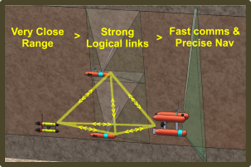
\includegraphics[width=0.5\textwidth]{Images/projects/Picture2.png}
    \caption{Morph Project}
    \label{fig:morph}
\end{figure}
    
\begin{figure}[h!]
    \centering
    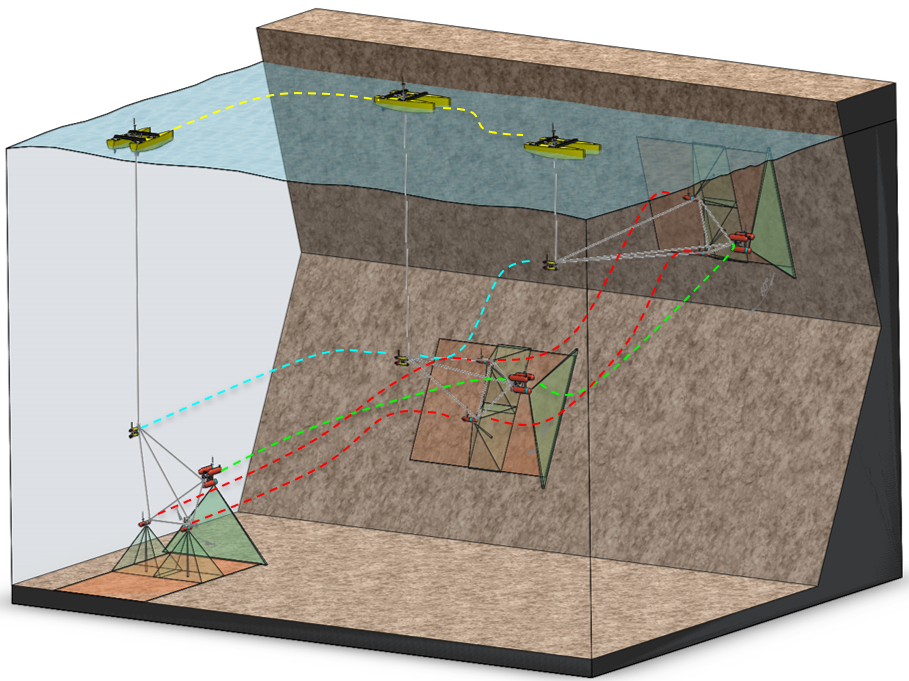
\includegraphics[width=0.6\textwidth]{Images/projects/Picture1.png}
    \caption{Morph Project}
    \label{fig:morph}
\end{figure}


\section{Background}

\par The work discussed in this thesis emphasises in the use of motion planning for multiple cooperative vehicles. Motion Planning, as the name suggests, consists in planning motion for robots, such as mobile vehicles or robotic arms. The choice of control law, i. e., the input which is provided to a robot, will result in a motion which is optimal according to a certain criteria. This criteria could be, for example, minimising time or consumed fuel. Formulisation of such a problem is known as an optimal control problem.
\par There are two main families of techniques for solving optimal control problems: direct methods and indirect methods.
\par Indirect methods 
% https://math.stackexchange.com/questions/946343/optimal-control-difference-between-indirect-direct-approaches
\par Direct methods in optimal control convert the optimal control problem into an optimization problem of a standard form and then using a nonlinear program to solve that optimization problem. 

\par Different models to represent vehicles exist such as a Dubin's car, Medusa Model.
% \par There are two main strategies for motion planning, one is \ac{TT} and the other is \ac{PF}. The first requires a vehicle to follow a path parameterized in space and time, whereas the latter only requires the vehicle to follow a path parameterized in space. Regardless of the strategy, the resulting evirnomental and dynamic constraints are met. Environmental constraints may include inter vehicular constraints, obstacle avoidance. Dynamic constraints include respecting maximum torque, acceleration, velocity and others for each vehicle.



\section{Objectives}


\par There are several ways to obtain a trajectory, for example, single and multiple shooting, collocation and quadratic programming. However, polynomial methods based on Bezier curves are particularly advantageous because they have favourable geometric properties which allow the efficient computation of the minimum distance between trajectories. As the complexity of the polynomials increases, the solutions converge to the optimal.
\par The cost can be constructed based on several criteria such as time and consumed energy. For \textit{cooperative} motion planning, the cost will have to be constructed differently because it will have to take into account the motion of the multiple vehicles at once, in particular, possible inter-vehicle collision.


\begin{itemize}
    \item test some methods for obstacle avoidance
    \item compare some different parameterization methodoligies
    \item analize the complexity of increasing order and number of vehicles
\end{itemize}

\todo{explain that we want to show that bernstein methods work for non differentially flat models like medusa}

\par This 

\section{Overview}

\par A path is a parameterized curve, which is a function that maps a segment $[a,b]$ to $\mathbb{R}^3$. If the parameter of path $p$ is time or a function of time, the map $t\mapsto p(t)$ is called a trajectory.
\par \ac{PF} refers to the problem of making vehicles converge to and follow a path with no explicit temporal schedule while \ac{TT} is the problem of making a vehicle track a trajectory such that both spacial and temporal schedules are satisfied simultaneously.
\par Motion Planning consists in the design of trajectories for different kinds of systems that can later be tracked.
\par A trajectory is the path that an object with mass in motion follows through space as a function of time. Trajectory tracking is the 
\par The objective of motion planning is to find a trajectory to be tracked by a robot in an optimal way, based on a "cost function".
\par 


%\section{Optimization methods: a brief survey}
\section{Problem Statement}



\par Discuss the difference between trajectory tracking and motion planning
\par Discuss the different models for vehicles
\par Maybe discuss optimization software like fmincon (J Garcia does this)
\par Maybe discuss the use of log barrier function
% \subsection{Polynomial methods}
% \subsection{Shooting}
% \section{}



\section{Thesis Outline}


% to use refs: \ref{chap:available_methods} try \Cref{} too. it works for more than just  chapters
\par In chapter \ref{chap:theory}, an overview of the different available numerical methods for the motion planning for a single vehicle will be presented. \todo{exapnd}
\par In chapter \ref{chap:autonomousvehiclemodels}, an overview of different vehicle models is presented. \todo{expand}
\par In chapter \ref{chap:implementation}, a discussion of the code structure is discussed, along with the choice of optimisation algorithms. \todo{exapnd}
\par In chapter \ref{chap:results}, some results are presented. \todo{exapnd}
\par In chapger \ref{chap:conclusion}, the conclusion is made. \todo{exapnd}

This will be followed, in chapter , by application examples for a double integrator in 1 and 2 dimensions that capture the dynamics of a single vehicle. In chapter , some considerations for the control of multiple cooperative vehicles will be presented. The report will be concluded with a final overview of the different methods considered and a plan for the project's work will be defined.

% If Printing on DOUBLE SIDED pages, the second page should be white.
% Otherwise, comment the following command:
\cleardoublepage
%
%Chapter 2
\fancychapter{Existing Trajectory optimization Methods for Motion Planning}%
\cleardoublepage%
% The following line allows to ref this chapter
\label{chap:theory}
%\todo[color=green!40, author=Thomas, fancyline]{choose best title for chapter}{}

\par In this chapter, Direct Methods for trajectory optimization will be reviewed. These methods are generic, i.e., they can be applied to a wide range of dynamic systems. Here, these methods are applied to the control of a vehicle in both one and two dimensions. A good understanding of motion planning for single vehicles will be necessary before extending to multiple vehicles.

\section{The Optimization Problem}
\label{sec:optimprob_intro}

\par Motion planning for a single vehicle can be cast in the form of an optimal control problem of the form (see \cite{diehl2006fast})

\begin{equation}
    \begin{aligned}
    & \underset{x(.),u(.)}{\text{minimise}} && J = \int_0^T L(x(t),u(t))dt + \Psi (x(T)) \ dt\\
    & \text{subject to}  && x(0) = x_0, \\
        & && \dot{x} = f(x(t), u(t)), &&& t \in [0,T] \\ % &&&& \text{(fixed initial value)} \\
        & && h(x(t),u(t)) \geq 0, &&&  t \in [0,T] \\ % &&&& \text{(ODE Model)}\\
        & && r(x(T)) = 0 % &&&& \text{(terminal constraints)} &&&&&
    \end{aligned}
    \label{eq:general_cost}
\end{equation}
where $x(t)$ is defined as $x:[0,T]\rightarrow \mathbb{R}^{n_x}$, $u(t)$ is defined as $u:[0,T]\rightarrow \mathbb{R}^{n_u}$, $f(x,t)$ is the system of equations for the dynamics, defined as $f:\mathbb{R}^{n_x}\times \mathbb{R}^{n_u}\rightarrow \mathbb{R}^{n_x}$, $x_0$ is the initial state, $h(x(t)$, $u(t))$ represents the path constraints, $r(x(T))=0$ the terminal constraints, $L(x(t),u(t))$ is the running cost, defined as $L:\mathbb{R}^{n_x}\times \mathbb{R}^{n_u}\rightarrow \mathbb{R}$, $\Psi(x(t))$ is the terminal cost defined as $\Psi:\mathbb{R}^{n_x} \rightarrow \mathbb{R}$ and finally $T$ is known as the time ”horizon”, i. e., no matter what motion planning algorithm is used, the produced control law will only be valid within time $t\in[0;T]$.

\par An example of a path constraint is to keep the minimum distance to a known obstacle bounded below by a desired safety distance. If $x$ encodes the position then $h(x)$ could be
\begin{equation}
    \label{eq:example_constr}
    h(x(t)) = \underset{t\in[0,T]}{\text{min}}\lVert x - p_0 \rVert - d_{\text{min}}
\end{equation}
where $p_0$ is the location of an obstacle's centre of mass and $d_{\text{min}}$ is the minimum accepted distance to that centre.

\par All of the available Direct Methods used in this Thesis have as an objective the formulation of a control law that optimises some form of the above cost function. These methods will be demonstrated with the control of a double integrator in 1-D and 2-D. A double integrator is a linear system where the second derivative of the position variable $y$, is the acceleration $a$, that is,
\begin{equation}
    \ddot{y} = a
    \label{eq:basic_double_int}
\end{equation}
\par A general linear system is represented, in state-space form, by
\begin{equation}
    \dot{x} = Ax + Bu
    \label{eq:general_state_space}
\end{equation}
where $x = [x_1,\dots,x_{n_x}]^T$ is the state of the system and $u = [u_1,\dots,u_{n_u}]^T$ is the input. For the double integrator, the states and inputs are given by
\begin{equation}
\begin{cases}
    x_1 = y \\ x_2 = v \\ u = a
\end{cases}
\end{equation}
where $x_1$ and $x_2$ represent position and velocity, respectively, and $u$ is the acceleration. The system's dynamics then become
\begin{equation}
    \label{eq:dynamics_double_int}
    \begin{cases}
        \dot{x}_1 = x_2 \\
        \dot{x}_2 = u
    \end{cases}
\end{equation}
or
\begin{equation}
    \begin{bmatrix}
    \dot{x}_1 \\ \dot{x}_2
    \end{bmatrix} = 
    \begin{bmatrix} 0 & 1 \\ 0 & 0 \end{bmatrix} 
    \begin{bmatrix} x_1 \\ x_2 \end{bmatrix} + 
    \begin{bmatrix} 0 \\ 1 \end{bmatrix} u
    \label{eq:state_space_double_int}
\end{equation}
in matrix form, which means matrices $A$ and $B$ of equation \ref{eq:general_state_space} are given by
\begin{equation}
    A = \begin{bmatrix} 0 & 1 \\ 0 & 0 \end{bmatrix}, \qquad B = \begin{bmatrix} 0 \\ 1 \end{bmatrix}
    \label{eq:A_and_B}
\end{equation}.

\par The cost function \ref{eq:general_cost} will be simplified to
\begin{equation}
    J = \int_0^\infty x_1^2 + x_2^2 + \rho u^2\  dt
    \label{eq:my_cost}
\end{equation}
where $\rho$ is a scalar that penalizes "energy" consumption.
\par This dynamic system is diferentially flat (see section \ref{sec:differentiallyflatsystems}) with $x_1$ as the flat output, because it is possible to express $x_2$ as a derivative of $x_1$ and $u$ as a double derivative of $x_1$.
\par Although this 1-D model is very simple, it can provide insight into real life applications. One obvious example is a train that follows a track. It cannot leave the track and so, environmental constraints, such as obstacles, cannot be fixed in time if they are between the train's initial and target position. A non-fixed constraint could be another train that is joining the same track, therefore, the first train cannot be at certain points at certain times.
\par The optimization problem \eqref{eq:general_cost}, is infinite dimensional because the solution will be a function of time, which has an infinite number of points. The following Direct Methods will replace the infinite number of points of the function by approximated functions which are parameterized by a finite number of variables.
\par Before presenting the Direct Methods, results of the application of the \acl{LQR} are presented. This is important as the results serve as baselines to compare with the Direct Methods. The \ac{LQR} is a feedback law which guarantees minimal cost for certain kinds of cost functionals.

\section{Linear Quadratic Regulator}
\label{sec:linearquadraticregulator}

\par A \acl{LQR} is a technique applicable to linear dynamic systems of the form
\begin{equation}
    \label{eq:dynamic_system}
    \dot{x} = A x + B
\end{equation}
using the same definitions as in section \ref{sec:optimprob_intro}.

\par The Linear Quadratic Regulator algorithm yields, under certain conditions, an appropriate state-feedback LQR controller that minimises a cost function of the form
\begin{equation}
    \label{eq:quadratic_cost}
    J = \int_0^\infty x^T Q x + u^T R u + 2x^T N u dt
\end{equation}

\par The control law is of the form
\begin{equation}
    \label{eq:feedback}
    u = -Kx
\end{equation}
where $K$ is given by
\begin{equation}
    \label{eq:k_expression}
    K = R^{-1} (B^T P(t) + N^T)
\end{equation}
where $P(t)$ is the solution of the differential Riccati equation \cite{riccati1724animadversiones}
\begin{equation}
    \label{eq:p_diff_expression}
    A^T P(t) + P(t) A - (P(t) B + N) R^{-1} (B^T P(t) + N^T) + Q = - \overline{P}(t)
\end{equation}
with appropriate boundary conditions.

\par For the situation where the time horizon $T$ is $\infty$, $P(t)$ will tend to a constant solution, $P$, and, as a result, $P$ is found by solving the continuous time algebraic Riccati equation 
\begin{equation}
    \label{eq:p_expression}
    A^T P + PA - (PB + N) R^{-1} (B^T P + N^T) + Q = 0
\end{equation}

%\par Note that the cost in this equation is for an infinite time horizon and for continuous-time linear systems given by \ref{eq:dynamic_system}. The feedback control law.

\par The solution provided by this algorithm will be optimal and unique if the following conditions are fulfilled:
\begin{itemize}
    \item $(A,B)$ is controllable;
    \item for a system output $y = C x$, with $Q=C^T C$, the pair $(A,C)$ is observable;
    \item $R>0$ and $Q>0$.
\end{itemize}

\par Control via LQR is in closed-loop form, which has the advantage of being robust against parameter uncertainty and reducing the effect of external disturbances. 
\par In order to visualise the resulting controlled double integrator evolves over time, the feedback law \eqref{eq:feedback} is fed into the system \eqref{eq:dynamic_system}, non zero initial conditions are provided, and the resulting \ac{IVP} is solved. In other words, the objective is to find the soltion to 
\begin{equation}
    \begin{aligned}
    & \dot{x} = (A-BK)x \\
    & \text{subject to} \quad x(0) = x_0
    \end{aligned}
    \label{eq:controlledlinearsystem}
\end{equation}
where $x_0$ is the initial conditions.

%\par The regulator parameters can only be obtained for a more specific subset of the cost functions of equation \ref{eq:general_cost}. These will be given in the form of equation \ref{eq:quadratic_cost}. Where Q and R are matrices.

%\par \texttt{Matlab} implements the solution of the quadratic regulator in the functions \texttt{lqr} (for continuous systems) and \texttt{dqlr} (for digital systems). % These functions calculate the solution to the Riccati equation.

\par Here an example of control of the double integrator is presented in the context of linear quadratic regulator theory. Here, the initial conditions, which will be the same for all the subsequent 1-dimensional examples throughout this chapter, are  given by
\begin{equation}
    \label{eq:initial_conds}
    x_0 = \begin{bmatrix} x_{1_0} \\ x_{2_0} \end{bmatrix} = \begin{bmatrix} 3 \\ 1 \end{bmatrix}
\end{equation}

\par Figure \ref{fig:solution_lqr} shows the of an \ac{LQR} controlled double integrator. The regulator used for this example was obtained with $Q = I$ and $R = \rho = 0.1$ as weights to obtain $K$ in equation \ref{eq:k_expression} so that the resulting cost matches \ref{eq:my_cost}.



%\begin{equation}
%    x = \begin{bmatrix}x_1 \\ x_2\end{bmatrix}, \qquad Q = \begin{bmatrix} 1 & 0 \\ 0 & 1 \end{bmatrix}, \qquad R = \rho, \qquad N = 0
%\end{equation}

\begin{figure}[h!]
\centering
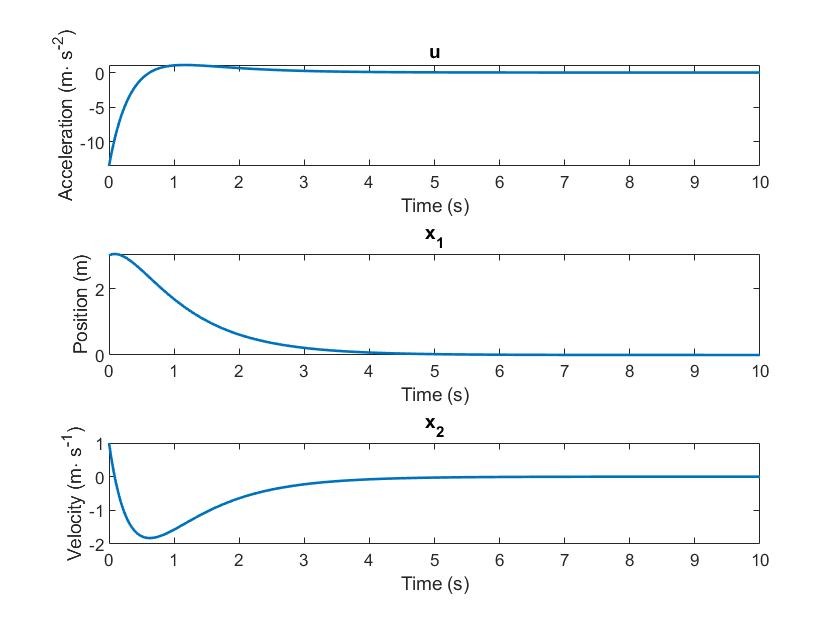
\includegraphics[width=0.8\textwidth]{Images/solution_lqr.jpg}
\caption{\acs{LQR}-Controlled Double Integrator Solution}
\label{fig:solution_lqr}
\end{figure}

\par It can be seen that all variables tend asymptotically to zero. It should be noted that after around 6 seconds the system can already be considered stationary.



\section{Single Shooting}
\label{sec:singleshooting}

\par Single Shooting is a direct method for motion planning. It consists of parameterising, for a given system, the control input signal $u(t)$ as a piece-wise constant function of time, as defined by 
\begin{equation}
    \label{eq:single_shooting}
    u(t) = q_i, \qquad t\in [t_i,t_{i+1}]
\end{equation}
where $q_i$ has the dimensions of the input, and the intervals $[t_i,t_{i+1}]$ denote the time-intervals between instants indexed by indices $i$ and $i+1$.

\par The following step consists of solving the following \ac{ODE}:
\begin{equation}
    \label{eq:ode_zoh}
    \begin{aligned}
        & x(0) = x_0, \\
        & \dot{x}(t) = f(x(t),u(t;q)), && t\in[0,T].
    \end{aligned}
\end{equation}
to obtain the time evolution of $x$.

\par With the obtained trajectories, the optimization problem (\ref{eq:general_cost}) can be extended and expressed as a function of the parameters $q=(q_0,q_1,\dots,q_{N-1})$ as optimization variables. The new optimization problem is written in the form  
\begin{equation}
    \begin{aligned}
    & \underset{q}{\text{minimise}} && \int_0^T L(x(t;q),u(t;q))dt + \Psi (x(T;q)) \ dt \\
    & \text{subject to}  && x(0) = x_0, \\
        & && \dot{x} = f(x(t), u(t)), &&& t \in [0,T]  \\
        & && h(x(t),u(t)) \geq 0, &&&  t \in [0,T]  \\
        & && r(x(T)) = 0
    \end{aligned}
    \label{eq:cost_zoh}
\end{equation}

\par This method can produce good results when a sufficiently low step duration is used. However, an important concern when compared to other methods is the computation time. Convergence for a good solution takes a long time because the number of parameters that are used is relatively large. With an increasing number of search parameters comes a increasingly bigger complexity and, because the cost can only be calculated for the completed trajectory, calculating the gradients with respect to each parameter can be very difficult.

\par Trajectory planning for the double integrator with single shooting will be unconstrained. This is because the solution produced by the optimization problem will shape $u$, which will have no influence on the problem's initial conditions. 
\par The solution for this unconstrained problem can be found using the Matlab function \texttt{fminsearch}.
\par During the optimization process, the variables $x_1$ and $x_2$ will be necessary for calculation of the cost. The integral \ref{eq:my_cost} can be easily calculated without ever having to obtain an explicit expression for signals $x_1$ and $x_2$. This is because $x_2$ will be continuous piece-wise straight lines (by integration of constants) and $x_1$ will be continuous piece-wise parabolas (by integration of straight lines).

\par Figure \ref{fig:solution_zoh} shows the solution of this shooting problem. The input $u$ has a total of 30 coefficients, each having a duration of $\SI{20}{\milli\second}$.

\begin{figure}[h!]
\centering
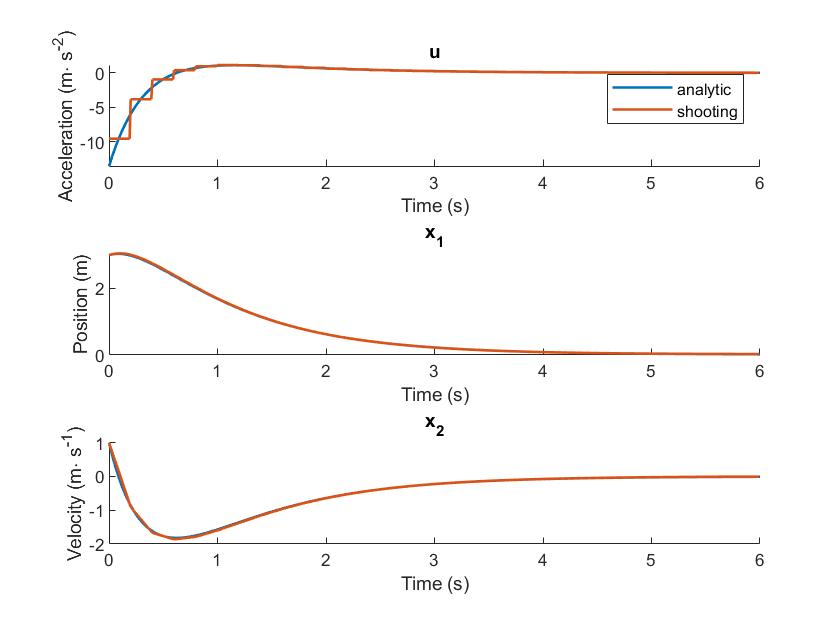
\includegraphics[width=0.8\textwidth]{Images/solution_zoh.jpg}
\caption{Direct optimization via a piecewise constant input.\\ Computation time: \SI{2.44}{\second}}
\label{fig:solution_zoh}
\end{figure}


\section{Multiple Shooting}

\par With multiple shooting, $u$ is parameterized in the same way as single shooting (see \ref{sec:singleshooting}). The main difference between multiple shooting and single shooting is that the ODE is calculated for each time interval separately. This ODE uses as initial value $s_i$ and is expressed as
\begin{equation}
    \dot{x}_i (t; s_i; q_i) = f(x_i(t;s_i,q_i),q_i), \qquad t\in [t_i; t_{i+1}]
    \label{eq:ode_multiple}
\end{equation}

\par Continuity of state $x$ for each time-step has to be assured. As a result, an equality constraint has to be added to the problem. This constraint is given by 
\begin{equation}
    \label{eq:shooting_constraint}
    s_{i+1} = x_i (t_{i+1}, s_i, q_i), \qquad i = 0,1,\dots, N-1
\end{equation}
where the path cost $l_i$ can now be calculated for each time interval $t \in [t_i; t_{i+1}]$ and is given by
\begin{equation}
    l_i(s_i;q_i) = \int_{t_i}^{t_{i+1}} L(x(t;s_i;q_i),q_i)dt 
\end{equation}

\par The optimization problem can now be redefined as
\begin{equation}
    \label{eq:cost_mul_shoot}
    \begin{aligned}
    & \underset{q,s}{\text{minimise}} && \sum_{i=0}^{N-1} l_i(s_i,q_i) + \psi (s_N) \\
    & \text{subject to}  && a(0) = x_0, \\
        & && s_{i+1} = x_i (t_{i+1}, s_i, q_i), &&& i = 0,1,\dots, N-1, \\
        & && h(s_i,q_i) \geq 0, &&& 1,\dots,N, \\
        & && r(x(T)) = 0
    \end{aligned}
\end{equation}

\par For a solution $u$ to be obtained with the same duration and order as in single shooting, the optimising algorithm will have to search through twice the amount of variables (an $s_i$ for every $q_i$). However, the larger search space will be sparse due to the presence of constraints, and, as a result, easier to solve, compared to the small and dense optimization problem produced by single shooting \cite{rao2009survey}.

\par Solutions for multiple shooting will be identical to single shooting and will differ only in computation time. As a result, examples with this method will not be given.

\section{Quadratic Programming}

\par Quadratic programming problems have the form
\begin{equation}
    \label{eq:gen_quad_prog}
    \begin{aligned}
    & \underset{\overline{x}(.)}{\text{minimise}} && \frac{1}{2} \overline{x}^T H \overline{x} + f^T  \\
    & \text{subject to} && A \cdot \overline{x} \leq b, \\
    & && Aeq \cdot \overline{x} = beq, \\
    & && lb \leq \overline{x} \leq ub
    \end{aligned}
\end{equation} 
and are not specifically designed to tackle motion planning problems. The first step in applying quadratic programming to optimal control problems is to discretise the system's dynamics. 
\par A discrete linear system can be represented as
\begin{equation}
    \label{eq:discrete_state_space} 
    \phi_{x_k} + \Gamma_{u_k} - x_{k+1} = 0,
\end{equation}
where $x_k$ and $u_k$ are the state and input, respectively, at discrete time $k$, and $\Phi$ and $\Gamma$ are state and input matrices, respectively of appropriate dimensions.
\par The cost function to optimise that is equivalent to $\ref{eq:quadratic_cost}$ is given by
\begin{equation}
    J_d = x_N^T Q x_N + \sum_{k=0}^{N-1} x_k^T Q x_k + u_k^T R u_k
    \label{eq:discrete_quad_cost}
\end{equation}
where the matrices $Q$ and $R$ will be identical to the continuous time problem.

\par The goal of the quadratic programming optimiser is to obtain values $x_k$ and $u_k$ for all discrete-times that minimise \ref{eq:discrete_quad_cost}. In order to formulate the optimization problem in the form of \ref{eq:gen_quad_prog}, all of the variables to optimise have to be flattened to the column vector \begin{equation}
    \label{eq:quad_prog_xbar}
    \overline{x} = \begin{bmatrix} x^0_1\ \dots \ x^0_n & u_1^0\ \dots\ u_m^0 & (\dots) & x_1^{N-1}\ \dots\ x_n^{N-1} & u_1^{N-1}\ \dots\ u_m^{N-1} &  x_1^N\ \dots\ x_n^N \end{bmatrix} ^T,
\end{equation}
where the superscript is the iteration number that goes from 0 to $N$, $n$ is the dimension of $x$ and $m$ is the dimension of $u$. There will be a total of $(N-1)(n+m)+n$ variables to optimise.
\par To optimise \ref{eq:discrete_quad_cost}, matrix $H$ will be constructed by repetition of matrices $Q$ and $R$ as follows
\begin{equation}
    \label{eq:quad_prog_h}
    H = \begin{bmatrix}
        [Q] & & & & & \\
        & [R] & & & &  \\
        & & \ddots & & & \\
        & & & [Q] & & \\
        & & & & [R] & \\
        & & & & & [Q]
    \end{bmatrix}
\end{equation}

\par The system dynamics \ref{eq:discrete_state_space} will impose "dynamic" linear constraints given by
\begin{equation}
    \label{eq:quad_prog_Aeq_dyn}
    \underbrace{\begin{bmatrix}
        [\phi] & \left[\Gamma\right] & \left[ -I \right] & & \ldots \\
        & & [\Phi] & [\Gamma] & \left[ -I \right] & \ldots \\
        \vdots & \vdots & \vdots & \vdots & \vdots & \ddots 
    \end{bmatrix}}_\text{Aeq (dynamics)}
    \overline{x} = \underbrace{\begin{bmatrix} 0 \\ 0 \\ 0 \\ \vdots \\ 0 \end{bmatrix}}_\text{beq dynamics}
\end{equation}
where $I$ is the identity matrix with size equal to the dimension of $x$.

\par The first and last samples of $x$ will be restricted to the initial and final conditions, $x_i$ and $x_f$
\begin{equation}
    \label{eq:quad_prog_Aeq_init}
    \underbrace{\begin{bmatrix} 
        1 & 0 & 0 & \ldots & 0 \\
        0 & 1 & 0 & \ldots & 0 
    \end{bmatrix}}_\text{Aeq (initial state)}
    \overline{x} = \underbrace{\mathbf{x}^i}_\text{beq (initial state)}
\end{equation}
\begin{equation}
    \label{eq:quad_prog_Aeq_final}
    \underbrace{\begin{bmatrix} 
        0 & \ldots & 0 & 1 & 0 \\
        0 & \ldots & 0 & 0 & 1 
    \end{bmatrix}}_\text{Aeq (final state)}
    \overline{x} = \underbrace{\mathbf{x}^f}_\text{beq (final state)}
\end{equation}

\par The final matrices $Aeq$ and $beq$ that will be inserted into in the optimization software will be given by

\begin{equation}
    \label{eq:quad_prog_Aeq_total}
    \underbrace{\begin{bmatrix}
        \text{Aeq (dynamics)} \\ \text{Aeq (initial state)} \\ \text{Aeq (final state)}
        \end{bmatrix}}_\text{Aeq}
    \overline{x} =
    \underbrace{\begin{bmatrix}
        \vec{0} \\ x^i \\ x^f
        \end{bmatrix}}_\text{beq}
\end{equation}

\par An additional inequality constraint may be used to bound values of $\overline{x}$. These are coded in the $lb$ and $ub$ vectors which correspond to the lower bound and upper bounds for $\overline{x}$. Later, in the application examples, this will be used to bound the values of $u$.


\par In order to control the double integrator using quadratic programming techniques, the system's discrete-time equivalent will have to be obtained first. Matrices $\Phi$ and $\Gamma$ can be obtained via the Matlab function \texttt{c2d}. $H$ will be as described with $Q$ and $R$ identical to the analytical solutions; $f$ will be zero because there are no non-squared components of the cost function. Figure \ref{fig:solution_quad_prog_un} shows the solution of the quadratic problem for an unconstrained input and identical initial conditions to the analytical example were used.

%Within the context of motion control, these can be used to bound the input $u$, which, in this case, corresponds to leaving every corresponding variable of $\overline{x}$ to $U_{\text{max}}$ or $U_{\text{min}}$ and all others to $\pm \infty$ as shown in \ref{eq:quad_prog_ineq_constr}.
\par Figure \ref{fig:solution_quad_prog_con} shows the solution to a problem where $u$ is bounded by
\begin{equation}
\label{eq:quad_prog_ineq_constr}
\begin{gathered}
    ub = U_{\text{max}} \begin{bmatrix} \infty & \infty & 1 & \ldots & \infty & \infty & 1 & \infty & \infty \end{bmatrix} \\
    lb = U_{\text{min}} \begin{bmatrix} \infty & \infty & 1 & \ldots & \infty & \infty & 1 & \infty & \infty \end{bmatrix} 
\end{gathered}
\end{equation}
where $U_{\text{max}}$ and $U_{\text{min}}$ are given are given by $\pm 1$. Here we can see a clear saturation on the input up to time $\SI{2.5}{\second}$ after which the system evolves like in the unconstrained example.

\begin{figure}[h!]
\centering
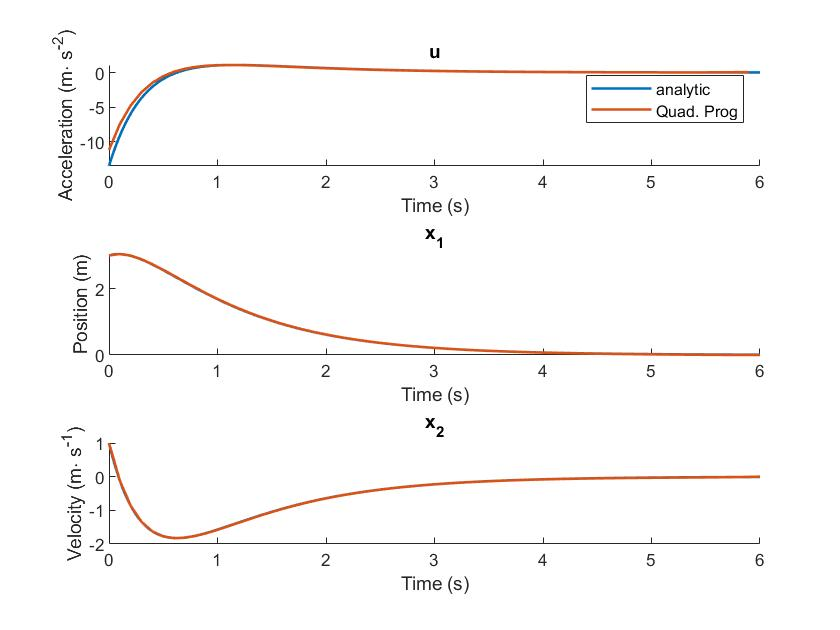
\includegraphics[width=0.75\textwidth]{Images/quad_prog_unconstrained.jpg}
\caption{Quadratic Programming solution}
\label{fig:solution_quad_prog_un}
\end{figure}


\begin{figure}[h!]
\centering
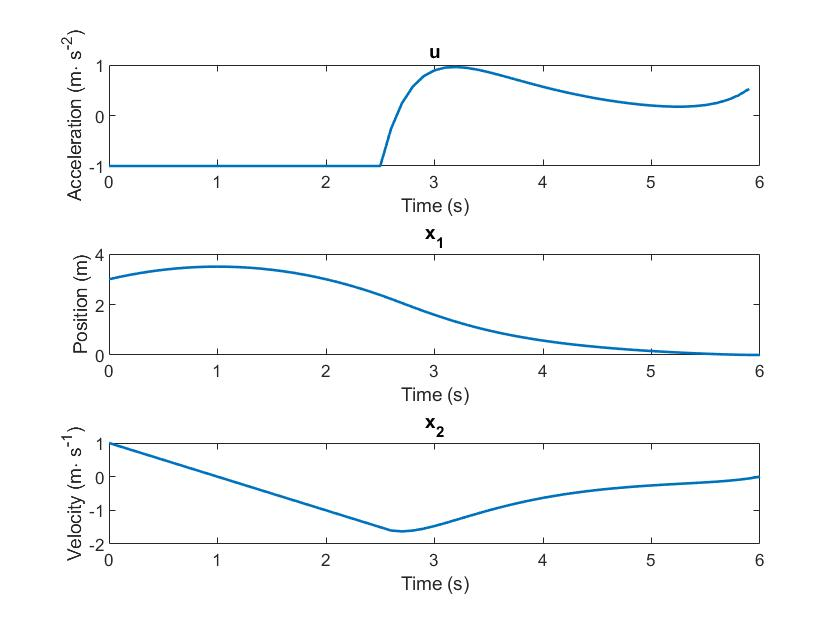
\includegraphics[width=0.75\textwidth]{Images/quad_prog_constrained.jpg}
\caption{Quadratic Programming solution with bounded input}
\label{fig:solution_quad_prog_con}
\end{figure}


\section{Monomial Polynomials}

\par Another way to describe trajectories is by using polynomials. If an optimal trajectory can be modelled by a polynomial, then it can be parameterized in terms of the polynomial's coefficients. As a result, the optimization problem tends to have a much smaller search space compared to, for example, shooting methods because with a relatively low order of polynomial, a whole trajectory over time $t\in [0,T]$ can be obtained will a relatively good cost. 
\par Polynomial methods are especially suited to deal with \textit{differentially flat systems} (see section \ref{sec:differentiallyflatsystems}). In differentially flat systems, the state and input variables can be directly expressed, without integrating any differential equation, in terms of the flat output and a finite number of its derivatives \cite{fliess1995flatness}. This means that with coefficients that describe just the flat output it is possible to describe all of the other variables of the system, thus resulting in a 

\par The solution provided by the Matlab function \texttt{fmincon} for the same double integrator problem of section \ref{sec:linearquadraticregulator} with this method will be a polynomial $\overline{p}$ for $x_1$. Once the optimal coefficients have been obtained the trajectories for $x_1$, $x_2$ and $u$ can be obtained by polynomial derivation and evaluation. This is possible because the system is differentially flat. These polynomials are related in the system of equations
\begin{equation}
    \label{eq:polys_of_double_integrator}
    \begin{cases}
        u (t) = a_0 + a_1 t + a_2 t^2 + \ (\dots) \\
        x_2 (t) = v_0 + a_0 t + \frac{a_1}{2} t^2 + \frac{a_2}{3} t^3 + \ (\dots)  \\
        x_1 (t) = p_0 + v_0 t + \frac{a_0}{2} t^2 + \frac{a_1}{6} t^3 + \frac{a_2}{12} t^4 + \ (\dots)
    \end{cases}
\end{equation}
 The cost function will be the same as the one used for the analytic method, and with the same initial conditions (see \ref{eq:my_cost} and \ref{eq:initial_conds}).
\par Figure \ref{fig:solution_pol} shows the solution of a polynomial optimization problem for a polynomial of order 7. Higher orders where attempted but take too long to converge. %Here, the variable to optimise $\overline{p}$ contains the coefficients that describes $x_1$. Because the system is deferentially flat, both $x_2$ and $u$ can be obtained as a function of $\overline{p}$  and will also be polynomials.


\par In order to guarantee the initial and final conditions of the state variable $x$, the linear constraint that has to be introduced is given by
\begin{equation}
    \label{eq:pol_equality}
    \underbrace{\begin{bmatrix}
    0 & 0 & \dots & 0 & 1 \\
    0 & 0 & \dots & 1 & 0 \\
    T^N & T^{N-1} & \dots & T & 0 
    \end{bmatrix}}_\text{Aeq} \overline{p}  =
    \underbrace{\begin{bmatrix} x_1^i \\ x_2^i        \\ 0 \end{bmatrix}}_\text{beq}
\end{equation}


\begin{figure}[h!]
\centering
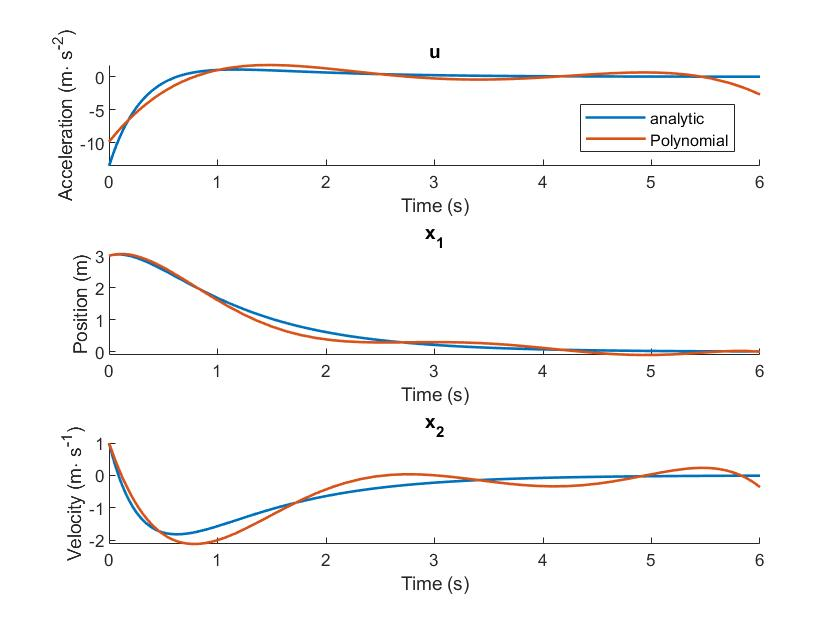
\includegraphics[width=0.8\textwidth]{Images/solution_pol.jpg}
\caption{Direct optimization with Polynomials. \\ Polynomial order: 7. \\
Computation time: \SI{1.33}{\second}}
\label{fig:solution_pol}
\end{figure}



\section{Bezier Curves}
\label{sec:bezcurves}
\par A Bezier curve is a parametric curve used in computer graphics and related fields. The curve, is named after Pierre Bezier, who used it in the 1960s for designing curves for the bodywork of Renault cars \cite{hazewinkelmichiel1997}.  Other uses include the design of computer fonts and animation \cite{hazewinkelmichiel1997}. 
The mathematical basis for Bezier curves, the Bernstein polynomials, was established in 1912, but the polynomials were not applied to graphics until some 50 years later when mathematician Paul de Casteljau in 1959 developed de Casteljau's algorithm, a numerically stable method for evaluating the curves, and became the first to apply them to computer-aided design at French auto-maker Citroen \cite{GeraldFarin2002}. 

\par What follows is a brief summary of the type of Bernstein polynomials that are exploited in this study.

\par A Bernstein polynomial is given by % represented as
\begin{equation}
    \label{eq:bern_pol}
    P(\tau) = \sum_{k=0}^n \overline{p}_k B_{k,n} (\tau), \qquad \tau\in [0,1]
\end{equation}
where $n$ is the order of the polynomial and $\tau$ is the time contraction of $t$, given by 
\begin{equation}
    \tau = \frac{t}{T}, \qquad t\in [0,T].
    \label{eq:time_delay}
\end{equation}
\par The $p_k$ are the polynomial coefficients or \textit{control points}, and $b_k^n$ are the \textit{Bernstein Basis}, given by 
\begin{equation}
	B^n_k {(\tau)} = \binom{n}{k} {(1 - \tau)}^{n-k} \tau^k
    \label{eq:bern_basis}
\end{equation}
As a result, a Bernstein polynomial of order $n$ is a linear combination of $(n+1)$ Bernstein basis with weights given by $p_k$. The Bernstein Basis, as a function of $\tau$, for 6 different orders, $n$, are shown in figure \ref{fig:bernsteinbasis}.

\begin{figure}[h!]
\centering
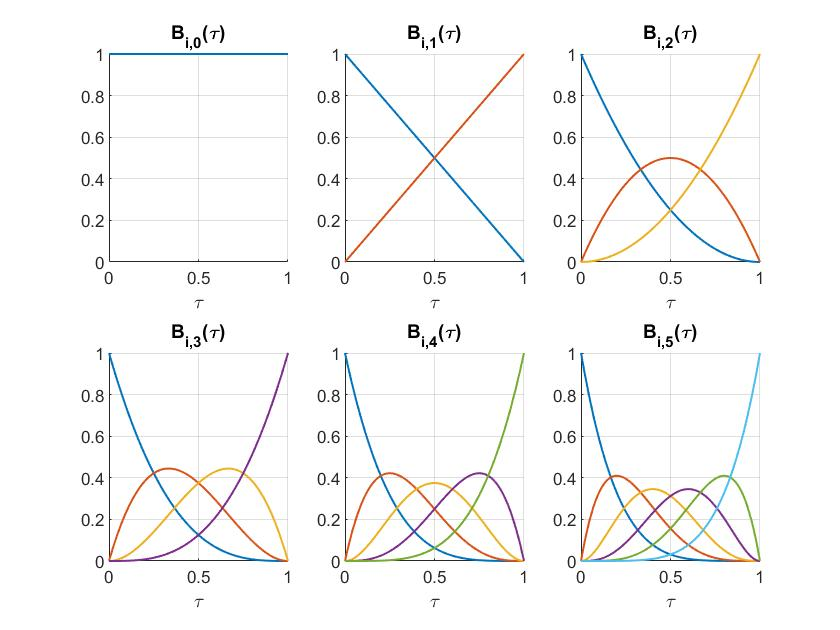
\includegraphics[width=0.8\textwidth]{Images/bernstein_basis.jpg}
\caption{Representation of the Bernstein Basis for $\tau \in [0,1]$ for orders $n=0\cdots 5$}
\label{fig:bernsteinbasis}
\end{figure}

\par For a polynomial of order $n$, the $i \in {0 .. n}$ control points can be represented as a vector on a vector $p$. For example, if $p$ is given by 
\begin{equation}
    \overline{p} = \begin{bmatrix}0\\ 0.5\\ 1\\ 0.7\\ 0.3\\ -0.7\\ -1\\ -0.5\\ -0.1\end{bmatrix},
\end{equation}
the plot of the polynomial given by these coefficients is shown in figure \ref{fig:generic_bezier}. The control points on vector $p$ are plotted along time in equidistant time nodes. What can be seen is that the control points "attract" the curve towards themselves.

\begin{figure}[h!]
\centering
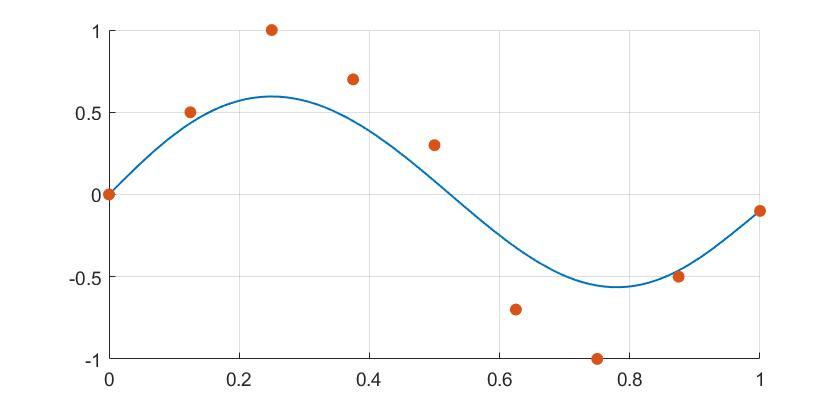
\includegraphics[width=0.8\textwidth]{Images/generic_bezier.jpg}
\caption{A Bernstein Polynomial}
\label{fig:generic_bezier}
\end{figure}


\par Two or three Bernstein polynomials of the same order, i.e., same number of control points, can be plotted against each other within the time domain $\tau \in [0,1]$. The control points of the curves together form $n+1$ points in two or three dimensions. These two or three dimension polynomials are also known as Bezier curves. Figure \ref{fig:generic_bezier} shows a 2-D Bezier Curve, the control points which resulted in it are plotted too. The control points for this curve had a specific order on the underlying Bernstein Polynomial. Changing the oder of the control points on the polynomial will, as a result, produce a different Bezier curve, such as the one in figure \ref{fig:generic_bezier2D_reordered}, despite the control points being the same on the 2-D plot.

\begin{figure}[h!]
\centering
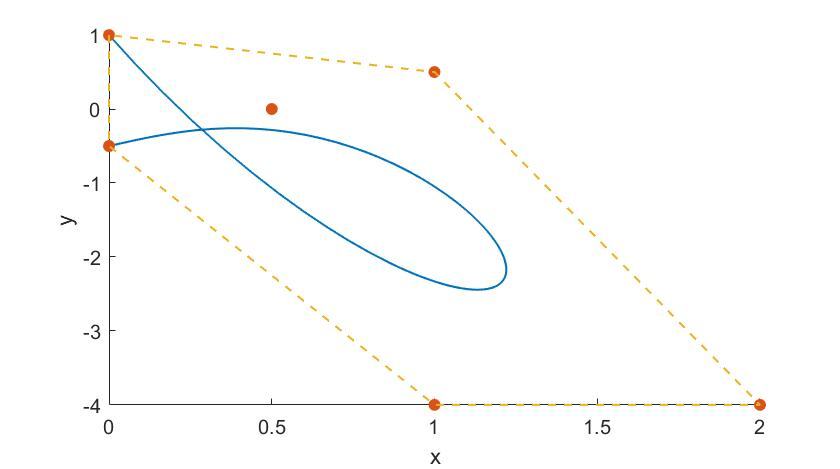
\includegraphics[width=0.8\textwidth]{Images/generic_bezier2D.jpg}
\caption{A 2-D Bernstein Polynomial}
\label{fig:generic_bezier2D}
\end{figure}

\begin{figure}[h!]
\centering
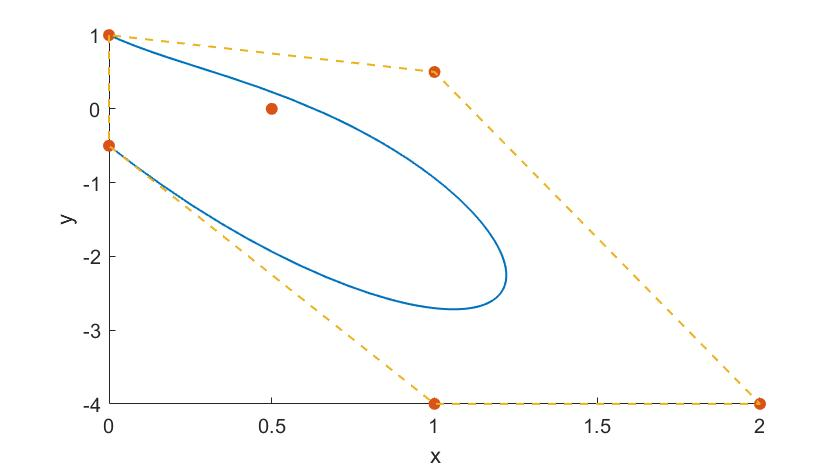
\includegraphics[width=0.8\textwidth]{Images/generic_bezier2D_reordered.jpg}
\caption{A 2-D Bernstein Polynomial with Reordered Control Points}
\label{fig:generic_bezier2D_reordered}
\end{figure}


\par One property than can be observed in figure~\ref{fig:generic_bezier} is that, within the domain $t \in [0,T]$, the polynomial is limited by a convex hull \cite{cichella2018bernstein} formed by the control points.
\par The initial and final values of $P(t)$ in the interval $[0,T]$ are given by
\begin{equation}
    \label{eq:bern_in_fin}
    \begin{gathered}
        P(0) = p_{n,0} \\
        P(T) = p_{n,n}
    \end{gathered}
\end{equation}
and the derivative and integral are given by 
\begin{equation}
    \label{eq:bern_deriv}
    \dot{P}(t) = \frac{n}{T} \sum_{k=0}^{n-1} (p_{k+1,n} - p_{k,n}) B_{k,n-1}(t)
\end{equation}
\begin{equation}
    \label{eq:bern_int}
    \int_0^T P(t)dt = \frac{T}{n+1} \sum_{k=0}^{n} p_{k,n}
\end{equation}

\par The control points for the derivative of a bernstein polynomial can be obtained my a multiplication of a derivation matrix by the control points of the original curve stored in the column vector, with the matrix given by 
\begin{equation}
    \boldsymbol{D}_{N-1} = 
    \begin{bmatrix}
        -\frac{N}{T} & \frac{N}{T} & 0 & \ldots & & 0 \\
        0 & -\frac{N}{T} & \frac{N}{T} & \ldots & & 0 \\
        \vdots &  \ddots & \ddots & \ddots & &   \\
        0 & & \ldots & & -\frac{N}{T} & \frac{N}{T}
    \end{bmatrix} \in \mathbb{R}^{(N+1)\times N}
    \label{eq:bernderivmat}
\end{equation}

\par The control points of the Anti-Derivative/Primitive can be obtained similarly to the derivation by multiplying the control points to a primitive matrix \cite{privateconversationprimitive}, and adding a vector:
\begin{equation}
    p = A \cdot \dot{p}  + p_0
\end{equation}
where $p_0$ is the initial values of $P$ and the matrix A is given by 
\begin{equation}
    \boldsymbol{A}_{N+1} = \begin{bmatrix}
        0 & 0 & \ldots & 0 & 0 \\
        \frac{T}{N+1} & 0 & \ldots & 0 & 0 \\
        \frac{T}{N+1} & \frac{T}{N+1} & \ldots & 0 & 0 \\
        \vdots & \ddots & \ddots & \ddots & \\
        \frac{T}{N+1} & \frac{T}{N+1} & \ldots & \frac{T}{N+1} & \frac{T}{N+1} \\
    \end{bmatrix}
\end{equation}

\par A Bernstein polynomial of degree $N$ and coefficients $p_{k,N}\in \mathbb{R}, k = 0,\dots,N$ can be expressed as a Bernstein polynomial of degree $M$ with $M>N$, with coefficients $p_{k,M} \in \mathbb{R}, k = 0,\dots,M$ given by 
\begin{equation}
    p_{k,M} = \sum_{j=\text{max}(0,k+M-N)}^{\text{min}(N,k)} \frac{{M-N \choose k-j}{N\choose j}}{{M\choose k}} p_{j,N} \in \mathbb{R}^n,
\end{equation}
which is known as degree elevation. In other words, it is possible find a polynomial with $M+1$ control points such that it's identical to a curve with order $N+1$ within time $t\in[0,T]$.
\par The control points for the degree elevation can also be obtained by multiplying the control points vector by a matrix $\boldsymbol{E}$ whose indices are given by 
\begin{equation}
    \label{eq:bernsteinelevindices}
    \boldsymbol{E}_{ij} = \frac{{N\choose j}{M-N\choose i-j}}{{M\choose i}}
\end{equation}


%\par The cost function, which will be the same as previous the previous examples, (\ref{eq:my_cost}). In order to calculate it and take, equations \ref{eq:bern_mul} and \ref{eq:bern_sum} will be necessesary for summation and addition of Bernstein polynomials, respectfully.
\par Multiplication and addition is given by
\begin{equation}
    \label{eq:bern_mul}
    f(t)g(t) = \sum^{m+n}_{i=0}  \left(\sum_{i=\text{max}(0,i-n)}^{\text{min}(m,i)} \frac{\binom{m}{j}\binom{n}{i-j}}{\binom{m+n}{i}} f_{j,m}g_{i-j,n}\right) B_{i,m+n}(t)
\end{equation}
\begin{equation}
    \label{eq:bern_sum}
    f(t)\pm g(t) = 
    \sum^{m}_{i=0}  \left(f_{i,n} \pm \sum_{j=\text{max}(0,i-m+n)}^{\text{min}(n,i)} \frac{\binom{n}{j}\binom{m-n}{i-j}}{\binom{m}{i}} g_{j,n}\right) B_{i,m+n}(t)
\end{equation}

\par The De Casteljau's algorithm \cite{shene2012finding} is a recursive method to evaluate polynomials in Bernstein form. A geometric interpretation of this algorithm presented as follows:
\begin{enumerate}
    \item Connect the consecutive control points in order to create the control polygon of the curve;
	\item Subdivide each line segment of this polygon with the ratio $t:(1-t)$ and connect the obtained points which results in a new polygon with one fewer control points;
    \item Repeat the process until a single point is achieved – this is the point of the curve corresponding to the parameter $t$.
\end{enumerate}

Figure~\ref{fig:deCasteljau} illustrates the breakdown of the control points into polygons and sub polygons. 
\par The evaluation of the curve can be carried out analytically. For a Bernstein Polynomial $\boldsymbol{x}_N:[0,t_f]\rightarrow \mathbb{R}^n$, and a scaler $t_{div}\in [0,t_f]$, the Bernstein polynomial at $t_{div}$ can be computed using the following recursive relation:
\begin{equation}
\begin{gathered}
    \overline{\boldsymbol{x}}^{[0]}_{i,N} = \overline{\boldsymbol{x}}_{i,N},\quad i=0,\dots, N  \\
    \overline{\boldsymbol{x}}^{[j]}_{i,N} = \overline{\boldsymbol{x}}^{[j-1]}_{i,N} \frac{t_f-t_{div}}{t_f} + \overline{\boldsymbol{x}}^{[j-1]}_{i+1,N} \frac{t_{div}}{t_f}
\end{gathered}
\end{equation}
with $i=0,\dots, N-j$, and $j=1,\dots, N$. Then, the Bernstein polynomial evaluated at $t_{div}$ is given by
\begin{equation}
    \overline{\boldsymbol{x}}_N(t_{div}) = \overline{\boldsymbol{x}}_{0,N}^{[N]}.
\end{equation}
Moreover, the Bernstein polynomial can be subdivided at $t_{div}$ into two $N$th order Bernstein polynomial with Bernstein coefficients
\begin{equation}
    \overline{\boldsymbol{x}}^{[0]}_{0,N}, \overline{\boldsymbol{x}}^{[1]}_{0,N}, \dots, \overline{\boldsymbol{x}}^{[N]}_{0,N}, \quad \text{and}\quad \overline{\boldsymbol{x}}^{[N]}_{0,N}, \overline{\boldsymbol{x}}^{[N-1]}_{0,N}, \dots, \overline{\boldsymbol{x}}^{[0]}_{0,N}.
\end{equation}

\begin{figure}[h!]
\centering

\includegraphics[width=0.8\textwidth]{Images/deCasteljau.png}
\caption{Visual representation of the De Casteljau algorithm}
\label{fig:deCasteljau}
\end{figure}

%\par A numerically stable method to evaluate Bernstein polynomials exists and is known as the \textit{deCasteljau} algorithm;

%\begin{description}
%    \item[$L$] is the lagrangian
%    \item[$\Psi$] is the terminal cost
%    \item[$f(x,t)$] is the dynamic model   
%\end{description}

The convex hull property of these polynomials will prove useful in an algorithm that calculates distance between curves, which will be used in deconfliction of trajectories in multiple vehicle control. By just knowing the position of the control points in the space, it is possible to guarantee constraint satisfaction in the whole trajectory and not just in the control points.

\par Just as with monomial polynomials, when these Bernstein polynomials are applied to differentially flat systems, a reduction of the number of parameters to optimise is possible because with just a flat output, all state variables can be derived. If the system is not differentially flat, then parameters for all state variables need to be defined and optimised but will be subject to the constrained imposed by the system's dynamics.
%The optimization problems developed for motion planning in this study center around the use of what is known as Bernstein polynomials.

\par The solution obtained by the Matlab function \texttt{fmincon} for the same double integrator problem of section \ref{sec:linearquadraticregulator} with this Bernstein polynomial based approach will provide the coefficients $\overline{p}$ for the Bernstein polynomial of state variable $x_1$. 

\par Figure \ref{fig:bernstein_1d} shows the solution for the same quadratic optimization problem and with the same initial conditions as the previous sections. The red circles in the figure show the distribution of the obtained coefficients. The resulting polynomial has order 14.

\par In order to guarantee that the initial and final conditions are respected, the linear constraint that has to be introduced is given by
\begin{equation}
    \label{eq:bern_equality}
    \underbrace{\begin{bmatrix}
        1 & 0 & 0 & \dots & 0 \\
        \frac{n}{T} & -\frac{n}{T} & 0 & \dots & 0 \\
        0 & 0 & 0 & \dots & 1 \end{bmatrix}}_{\text{Aeq}_{\text{1D}}} \overline{p} =
    \underbrace{\begin{bmatrix}
        x_0^i \\ x_1^i \\ 0\end{bmatrix}}_{\text{beq}_{\text{1D}}}
\end{equation}


\begin{figure}[h!]
\centering
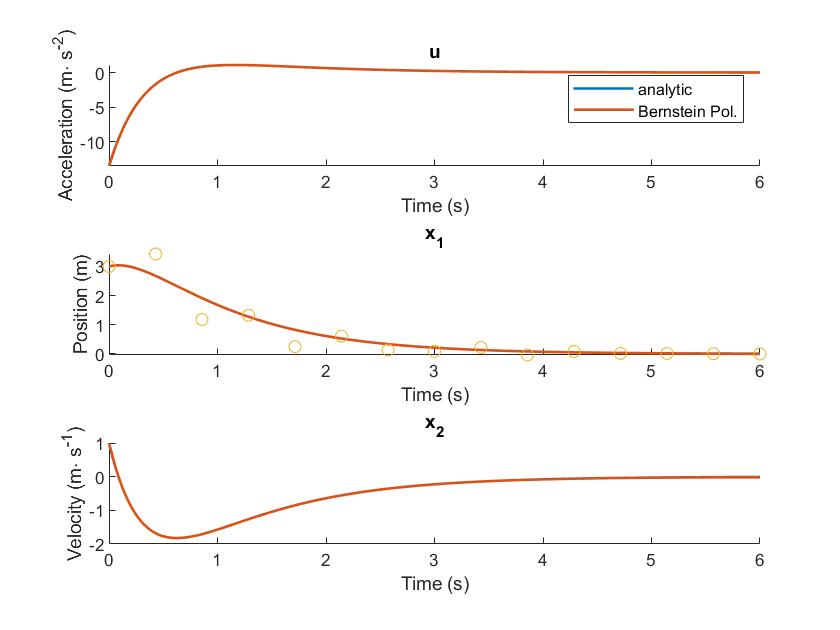
\includegraphics[width=0.8\textwidth]{Images/bernstein_1d.jpg}
\caption{Direct Bernstein Solution}
\label{fig:bernstein_1d}
\end{figure}

\section{Differentially Flat Systems}
\label{sec:differentiallyflatsystems}

\par A nonlinear system of the form
\begin{equation}
    \dot{x} = f(x(t),u(t)), \quad x(t) \in \mathbb{R}^n
\end{equation}
is said to be \textit{differentially flat} \cite{fliess1995flatness} or simply \textit{flat} if there exists a set of variables $y = (y_1, \dots, y_m)$ called the \textit{flat output}, such that
\begin{itemize}
    \item the components of $y$ are not differentially related over $\mathbb{R}$;
    \item every system variable, state or input, may be expressed as a function of the components of $y$ and a finite number of their time-derivatives, and 
    \item every component of $y$ may be expressed as a function of the system variables and of a finite number of their time-derivatives. 
\end{itemize}

\par The flat output has, in general, a clear physical interpretation and captures the fundamental properties of a given system and its determination allows to simplify considerably the control design. This implies that there is a fictitious \textit{flat output} that can explicitly express all states and inputs in terms of the flat output and a finite number of derivatives, thus reducing the number of parameters to be optimised.



\section{Remarks}

\par Out of all of the presented Direct Methods, the preferred is the Bernstein polynomials method because it provides fast solutions for the simple double integrator problem and, as will be seen in later chapters, will prove advantageous for differentially and non-differentially flat dynamic systems.

% If Printing on DOUBLE SIDED pages, the second page should be white.
% Otherwise, comment the following command:
\cleardoublepage
%
%Chapter 3
% #############################################################################
% This is Chapter 3
% !TEX root = ../main.tex
% #############################################################################
% Change the Name of the Chapter i the following line
\fancychapter{Autonomous Vehicle Models}
\cleardoublepage
% The following line allows to ref this chapter
\label{chap:autonomousvehiclemodels}

\par In this chapter equations that rule the motion of an autonomous marine vehicle are derived. But first, the coordinate frames will be defined (\ref{sec:refframes}). Then the general vehicle motion equations for the dubin's car (\ref{sec:dubincarequations}). Finally, the motion equations for the MEDUSA model are presented (the characterization of the vehicle MEDUSA (\ref{sec:medusamodelequations}). 
\par This chapter will focus primarily on dynamics in a two dimensional space.

\section{Reference Frames and Notaion}
\label{sec:refframes}


\par To derive the equations of motion for a marine vehicle it is standard practice to define two coordinate frames; Earth-fixed inertial frame $\{U\}$ composed by the orthonormal axes $\{x_U,y_U,z_U\}$ and the body-fixed frame $\{B\}$ composed by the axes $\{x_B,y_B,z_B\}$, as indicated in Figure \ref{fig:coordinate}.

\begin{itemize}
    \item $x_B$ is the longitudinal axis (directed from the stern to fore)
    \item $y_B$ is the transversal axis (directed from to starboard)
    \item $z_B$ is the normal axix (directed from top to bottom)
\end{itemize}

\par To simplify the model equations, the origin of the body-fixed frame is normally chosen to coincide with the centre of mass of the vehicle. The motion control of $\{B\}$ (that corresponds to the motion of the vehicle) is described relative to the intertial frame $\{U\}$.

\par In general, six independent coordinate are necessary to determine the evolution of the position and orientation (six \ac{DOF}), three position coordinates $(x,y,z)$ and using the Euler orientation angles $(\phi, \theta, \psi)$. The six motion components are difined as \textit{surge}, \textit{sway}, \textit{heave}, \textit{roll}, \textit{pitch}, and \textit{yaw}, and adopting the SNAME \footnote{The Society of Naval Architects \& Marine Engineers - http://www.sname.org/} notation it can be written as in the Table \ref{tab:coordinate_notation} or in a vectorial form: 
\begin{itemize}
    \item $\eta_1 = [x,y,z]^T$ - position of the origin of $\{B\}$ with respect to $\{U\}$
    \item $\eta_2 = [\phi, \theta, \psi]^T$ - orientation of $\{B\}$ with respect to $\{U\}$.
    \item $\nu_1 = [u,v,w]^T$ - linear velocity of the origin of $\{B\}$ relative to $\{U\}$, expressed in $\{B\}$.
    \item $\nu_2 = [p,q,r]^T$ - angular velocity of $\{B\}$ relative to $\{U\}$, expressed in $\{B\}$.
    \item $\tau_1 = [X,Y,Z]^T$ - actuating forces expressed in $\{B\}$.
    \item $\tau_2 = [K,M,N]^T$ - actuating moments expressed in $\{B\}$
\end{itemize}
In compact form yields
\begin{equation}
    \begin{cases}
        \eta = [\eta_1^T, \eta_2^T]^T \\
        \nu = [\nu_1^T, \nu_2^T]^T \\
        \tau_{RB} = [\tau_1^T, \tau_2^T]^T
    \end{cases}
\end{equation}

\begin{table}[h!]
\begin{tabular}{|l|l|l|l|}
\hline
\multicolumn{1}{|c|}{Degree of Freedom} &
  \multicolumn{1}{c|}{\begin{tabular}[c]{@{}c@{}}Forces and\\ moments\end{tabular}} &
  \multicolumn{1}{c|}{\begin{tabular}[c]{@{}c@{}}Linear and\\ angular velocities\end{tabular}} &
  \multicolumn{1}{c|}{\begin{tabular}[c]{@{}c@{}}Position and\\ Euler angles\end{tabular}} \\
\hline
1. Motion in the $x$-direction (surge) & $X$ & $u$ & $x$      \\
2. Motion in the $y$-direction (sway)  & $Y$ & $v$ & $y$      \\
3. Motion in the $z$-direction (heave) & $Z$ & $w$ & $z$      \\
4. Rotation about the $x$-axis (roll)  & $K$ & $p$ & $\phi$   \\
5. rotation about the $y$-axis (pitch) & $M$ & $q$ & $\theta$ \\
6. Rotation about the $z$-axis (yaw)   & $N$ & $r$ & $\psi$   \\
\hline
\end{tabular}
\caption{Notation used for marine vehicles}
\label{tab:coordinate_notation}
\end{table}

\begin{figure}[h!]
\centering
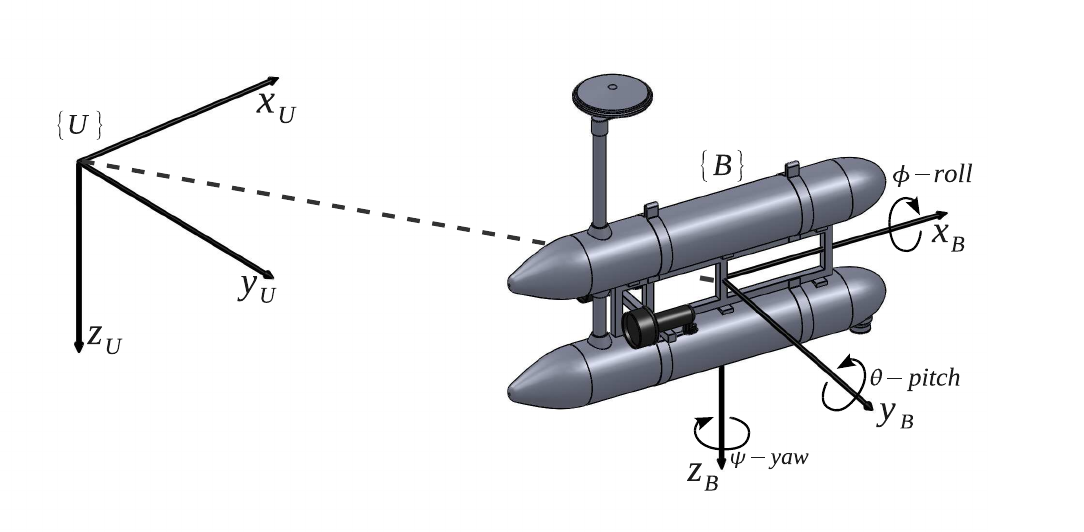
\includegraphics[width=0.8\textwidth]{Images/coordinate_frames.png}
\caption{Coordinate frames}
\label{fig:coordinate}
\end{figure}

\section{Medusa}
\label{sec:medusamodelequations}

\par The kinematics envolves only the gemotrical aspects of motion, and relates the velocities with poisiton. Using the coordinate frames notation in Section \ref{sec:refframes}, the kinematic equation can be expressed as
\begin{equation}
    \dot{\eta} = J(\eta)\nu
\end{equation}
with 
\begin{equation}
    J(\eta) = \begin{bmatrix}
        \prescript{U}{B}{R}
    \end{bmatrix}
\end{equation}
where
\begin{equation}
    \prescript{U}{B}{R(\Theta)} = \begin{bmatrix}
        c\psi c\theta & c\psi s\theta s\phi-s \psi c\phi & c\psi s\theta c\phi+s\psi s\phi \\
        s\psi c\theta & s\psi s\theta s\phi+c\psi c\phi & s\psi s\theta c\phi-c\psi s\phi \\
        -s\theta & c\theta s\phi & c\theta c\phi
    \end{bmatrix}, s\cdot = \sin(\cdot), c\cdot=\cos(\cdot)
\end{equation}
is the rotation matrix from $\{B\}$ to $\{U\}$, \cite{fossen2006nonlinear}, defined my means of three successive rotations ($zyx$-convention):

\begin{equation}
    \prescript{U}{B}{R(\Theta)} = R_{z,\psi}R_{y,\theta}R_{x,\phi}
\end{equation}
and
\begin{equation}
    T_{\Theta}(\Theta) = \begin{bmatrix}
        1 & s\phi\ t\theta & c\phi t\theta \\
        0 & c\phi & -s\phi \\
        0 & c\phi / c\theta & c\phi / c\theta 
    \end{bmatrix}, \theta \neq \pm 90º
\end{equation}

is the Euler attitude transformation matrix that relates the body-fixed angular velocities $(p, q, r)$ with the roll($\dot{\phi}$), pitch($\dot{\theta}$) and yaw($\dot{\psi}$) rates. Notice that $T_\Theta(\Theta)$ is not defined for the pitch angle $\theta = \pm90º$, resulting from using Euler angles to describe the vehicle’s motion. To avoid this singularity, one possibility is to use a quaternion representation \cite{fossen2006nonlinear}. However, due to physical restrictions, the vehicle will operate far from this singularity ($\theta\approx 0$ and $\psi \approx 0$) which implies that we can use the Euler representation.


\subsection{Dynamic equations}

Since the hydrodynamic forces and moments have simpler expressions if written in the body frame because they are generated by the relative motion between the body and the fluid, it is convenient to formulate Newton’s law in $\{B\}$ frame. In that case, the rigid-body equation can be expressed as

\begin{equation}
    M_{RB}\dot{\nu} + C_{RB}(\nu)\nu = \tau_{RB}
    \label{eq:rigid_body}
\end{equation}

where $M_{RB}$s the rigid body inertia matrix, $C_{RB}$ represents the Coriolis and centrifugal terms and $\tau_{RB}$ is a generalized vector of external forces and moments and can be decomposed as
 
\begin{equation}
    \tau_{RB} = \tau + \tau_A + \tau_D + \tau_R + \tau_{dist}
    \label{eq:tau_rb}
\end{equation}

where
\begin{enumerate}
    \item $\tau$ - Vector of forces and torques due to thrusters/surfaces which usually can be viewed as the control input
    \item $\tau_A$ + The force and moment vector due to the hydrodynamic added mass,
    \begin{equation}
        \tau_A = - M_A \dot{\nu} - C_A(\nu)\nu
        \label{eq:tau_a}
    \end{equation}
    \item $\tau_D$ - Hydrodynamics terms due to lift, drag, skin friction, etc.
    \begin{equation}
        \tau_D = - D(\nu)\nu
        \label{eq:tau_d}
    \end{equation}
    where $D(\nu)$ denotes the hydrodynamic damping matrix (positive definite).
    \item $\tau_R$ - Restoring forces and torques due to gravity and fluid density,
    \begin{equation}
        \tau_R = -g(\eta)
        \label{eq:tau_r}
    \end{equation}
    \item $\tau_{dist}$ - External disturbances: waves, wind, etc.
\end{enumerate}

\par Replacing \eqref{eq:tau_rb} on \eqref{eq:rigid_body}, taking into account \eqref{eq:tau_a}, \eqref{eq:tau_d}, the dynamic equations can
be written as

\begin{equation}
    \underbrace{M_{RB}\dot{\nu} + C_{RB}(\nu)\nu}_{\text{rigid-body terms}} + \underbrace{M_A(\dot{\nu}) + C_A(\nu)\nu + D(\nu)\nu}_{\text{hydrodynamic terms}} + \underbrace{g(\nu)}_{\text{restoring terms}} = \tau + \tau_{dist}
\end{equation}
which can be simplified to
\begin{equation}
    M\dot{\nu} + C(\nu)\nu + D(\nu)\nu + g(\nu) = \tau + \tau_{dist}
\end{equation}
where $M = M_{RB} + M_a$, $C(\nu) = C_{RB}(\nu) + C_A(\nu)$.

\subsection{Simplified Equations of Motion}

\par This thesis will focus on movement along a 2-D plane, therefor, the dynamics and kinematics can be simplified such that there are only three degrees of freedom $[x,y,\psi]$.
\par The kinematics with take the simpler form 

\begin{equation}
    \begin{gathered}
        \dot{x} = u \cos \psi - v \sin \psi, \\
        \dot{y} = u \sin \psi + v \cos \psi, \\
        \dot{\psi} = r.
    \end{gathered}
\end{equation}

\par $\tau_u$ and $\tau_r$ are the external force in $surge$ (common mode) and the external torque about the $z$-axis (differential mode between thrusters), respectively, which can by obtained by 
\begin{equation}
    \begin{gathered}
        \tau_u = F_{sb} + F_{ps}, \\
        \tau_r = l(F_{ps} - F_{sb})
    \end{gathered}
    \label{eq:simple_medusa_kinematics}
\end{equation}
where $F_{sb}$ and $F_{ps}$ are the starboard and port-side thruster forces, respectively, and $l$ is the length of the arm with respect to the centre of mass.
\par By neglecting roll, pitch and heave motion, the equations for $(u,v,r)$ without disturbances are
\begin{equation} 
    \begin{gathered}
        m_u\dot{u} - m_v v r + d_u u = \tau_u, \\
        m_v \dot{v} + m_u u r + d_v v = 0, \\
        m_r \dot{r} - m_{ub} u v + d_r r = \tau_r,
    \end{gathered}
    \label{eq:simple_medusa_dyamics}
\end{equation}
where
\begin{equation}
    \begin{gathered}
        m_u = m - X_{\dot{u}} \quad d_u = - X_u - X_{|u|u} |u| \\
        m_v = m - Y_{\dot{v}} \quad d_v = - Y_v - Y_{|v|v}|v| \\
        m_r = I_z - N_{\dot{r}} \quad d_r = - N_r - N_{|r|r}|r| \\
        m_{uv} = m_u - m_v
    \end{gathered}
    \label{eq:medusa_masses_and_drags}
\end{equation}


\par All the previous equations were expressed without considering the influence of external factors like ocean currents. If a constrant irrotational ocean current, $v_c$, is introduces, forming an angle $v = v_r+v_c$, where $u_r$ and $v_r$ are the components of the \acs{AUV} velocity with respect to the current and $u_c$ and $v_c$ are the components of the ocean current velocity in the body frame.
The previous dynamic equations \eqref{eq:simple_medusa_dyamics} become
\begin{equation}
    \begin{gathered}
        m_u\dot{u}-m_v(v_r+v_c)r+d_u u=\tau_u, \\
        m_v\dot{v}+m_u(u_r+u_c) r + d_v v=0, \\
        m_r\dot{r}-m_{ub}(u_r+u_c)(v_r+v_c)+d_r r=\tau_r,
    \end{gathered}
\end{equation}
where the expressions for masses and drags remain the same as in \eqref{eq:medusa_masses_and_drags}.


\subsection{\textit{Differentially flatify}}

\par Actually, the medusa model is differentially flat if $x$, $y$ and $\psi$ are to be considered the flat outputs.

The Remaining variables can be obtained by rearanging the kinematics:
\begin{equation}
\begin{split}
    & \begin{bmatrix}
        \dot{x} \\ \dot{y}
    \end{bmatrix} = 
    \begin{bmatrix}
        \cos(\psi) & - \sin(\psi) \\
        \sin(\psi) & \cos(\psi)
    \end{bmatrix} \cdot
    \begin{bmatrix}
        u \\ v
    \end{bmatrix} \Leftrightarrow  \\
    & \begin{bmatrix}
        u \\ v
    \end{bmatrix} = 
    \begin{bmatrix}
        \cos(\psi) & - \sin(\psi) \\
        \sin(\psi) & \cos(\psi)
    \end{bmatrix}^{-1} \cdot
    \begin{bmatrix}
        \dot{x} \\ \dot{y}
    \end{bmatrix} \Leftrightarrow \\
    & \begin{bmatrix}
        u \\ v
    \end{bmatrix} = 
    \begin{bmatrix}
        \cos(\psi) & \sin(\psi) \\
        - \sin(\psi) & \cos(\psi)
    \end{bmatrix} \cdot
    \begin{bmatrix}
        \dot{x} \\ \dot{y}
    \end{bmatrix}
\end{split}
\end{equation}
and the  inputs from the dynamics:
\begin{equation} 
    \begin{gathered}
        \tau_u = m_u\dot{u} - m_v v r + d_u u , \\
        \tau_r = m_r \dot{r} - m_{ub} u v + d_r r ,
    \end{gathered}
    \label{eq:rearaged_dynamics}
\end{equation}
 
\par These equations will always be valid, however, only for $x$, $y$ and $\psi$ that respect
\begin{equation}
    m_v \dot{v} + m_u u r + d_v v = 0
    \label{eq:onlymandatoryconstraint}
\end{equation}
because this equation is what guarantees $\tau_v = 0$. If $\tau_v \neq 0$, the vehicle will have to be fully actuated for the vehicle to follow it.



\section{Dubin Car}
\label{sec:dubincarequations}

\par The Medusa model can be even furhter simplified by a Dubin's Car.
\par In geometry, the term Dubins path typically refers to the shortest curve that connects two points in the two-dimensional Euclidean plane (i.e. x-y plane) with a constraint on the curvature of the path and with prescribed initial and terminal tangents to the path, and an assumption that the vehicle traveling the path can only travel forward \cite{wiki:dubincar}. 
\par A dubin's car is a simple model for a vehicle that transveses a dubin's path.
\par The main difference to the Medusa Model is that this will does not possess the possibility of side slip, therefor, less variables and dynamics equations will be necessary which will translate to a smaller computation time.

\par A simple kinematic car model for the systems is: 
\begin{equation}
    \begin{gathered}
        \dot{x} = u \cos \psi \\
        \dot{y} = u \sin \psi \\
        \dot{\psi} = \omega
    \end{gathered}
\end{equation}
where $(x,y)$ is the car's position, $\psi$ is the car's heading, $u$ is the car's speed, and $\omega$ is the car's turn rate.

\par The dynamics will be the simplest possible: basic accelerations.
\begin{equation}
    \begin{gathered}
        \dot{\omega} = r \\
        \dot{u} = a
    \end{gathered}
\end{equation}

\par This model is differentially flat because for any continuous $x$ and $y$, all of the other variables can be derived.
\par The tangent and rotational speeds can be obtained by
    
\begin{equation}
\begin{split}
    & \begin{bmatrix}
        \dot{x} \\ \dot{y}
    \end{bmatrix} = 
    \begin{bmatrix}
        \cos(\psi) & - \sin(\psi) \\
        \sin(\psi) & \cos(\psi)
    \end{bmatrix} \cdot
    \begin{bmatrix}
        u \\ 0
    \end{bmatrix} \Leftrightarrow  \\
    & \begin{bmatrix}
        u \\ 0
    \end{bmatrix} = 
    \begin{bmatrix}
        \cos(\psi) & - \sin(\psi) \\
        \sin(\psi) & \cos(\psi)
    \end{bmatrix}^{-1} \cdot
    \begin{bmatrix}
        \dot{x} \\ \dot{y}
    \end{bmatrix} \Leftrightarrow \\
    & \begin{bmatrix}
        u \\ 0
    \end{bmatrix} = 
    \begin{bmatrix}
        \cos(\psi) & \sin(\psi) \\
        - \sin(\psi) & \cos(\psi)
    \end{bmatrix} \cdot
    \begin{bmatrix}
        \dot{x} \\ \dot{y}
    \end{bmatrix}
\end{split}
\end{equation}
\par $\psi$ can be obtained by integrating $\omega$, however, because $\omega$ is not a flat output, $\psi$ is derived as
\begin{equation}
    \psi = \arctan{\frac{\dot{y}}{\dot{x}}}
\end{equation}
\par Finally, tangent acceleration, $\tau_1$ and torque, $\tau_2$ can be derived from $u$ and $\omega$:
\begin{equation}
    \tau_1 = \dot{u}
\end{equation}
\begin{equation}
    \tau_2 = \dot{\omega}
\end{equation}
which can be used as inputs to the system.

% If Printing on DOUBLE SIDED pages, the second page should be white.
% Otherwise, comment the following command:
\cleardoublepage
%
%Chapter 4
% #############################################################################
% This is Chapter 4
% !TEX root = ../main.tex
% #############################################################################
% Change the Name of the Chapter i the following line
\fancychapter{Implementation}
\cleardoublepage
% The following line allows to ref this chapter
\label{chap:implementation}

\par In this chapter, implementation of a Direct Methods based on the usage of Bernstein polynomails in both Matlab and Python will is described. This chapter focuses on formalising the optimisation problem for multiple vehicles. Once the optimisation problem is formalised, it can be solved by a whole range of non linear optimisation algorithms.

\section{The Optimisation Problem}
\label{sec:theoptproblem}

\par The Motion Planning problem for multiple vehicles that will be focused for the project consists in a go-to formation manoeuvre \cite{sabetghadam2018cooperative}. The go-to formation manoeuvre consists in the simultaneous arrival of a formation of vehicles to desired locations whilst simultaneously avoiding collisions between each other and the environment.

\par Just as for the case of optimisation for a single vehicle, motion planning for multiple vehicles will also be based on the minimisation of an appropriate cost function. This time, however, the cost will be the result of the sum of the costs of each individual vehicle and an added constraint will be necessary that will take into account inter vehicle collisions. 

\par The optimal control formulation for this motion planning problem is defined as
\begin{equation}
    \label{eq:multi_cost}
    \begin{aligned}
    & \underset{x^{[i]}(.),u^{[i]}(.),i= 1,\dots N_v}{\text{minimize}} && \int_0^T \sum_{i=1}^{N_v}  L_i (x^{[i]}(t),u^{[i]}(t))dt + \Psi (x^{[i]}(T)) \\
    & \text{subject to}  && x^{[i]}(0) = x_0^{[i]}, \\
        & && x^{[i]}(T) = x_f^{[i]}, \\
        & && \dot{x}^{[i]} = f^{[i]} (x^{[i]}(t), u^{[i]}(t)), &&& t \in [0,T]\\
        & && h(x(t),u(t)) \geq 0, \\
    \end{aligned}
\end{equation}
where $i=1\dots N_v$ refers to a vehicle out of $N_v$ vehicles.
\par This problem will also produce a solution within time horizon $t\in [0,T]$. Initial and terminal constraints will exist for every vehicle, as well as inter-vehicle constraints.

\par A problem that only has the integral term $\sum_{v=1}^{N_v} L_v(x^{(v)}(t),u^{(v)}(t))$ is said to be in \textit{Lagrange form}, a problem that optimises only the boundary objective $\sum_{v=1}^{N_v} \Psi_v(x(T))$ is said to be in \textit{Mayer form} and a problem with both terms is said to be in \textit{Bolza form}. An example where only the \text{Mayer form} would be necessary could be a situation where the desired destination of the vehicles does not have enough room for them all to be arranged in their desired positions. Therefore, the goal of the optimiser is to find the closest to the desired positions.

\par A direct method based on Bernstein polynomials is used, therefore, some or all of the state variables/inputs are approximated by polynomials, each with the same order $N$.

\par By using Bernstein approximation, all of the states and inputs for each vehicle combined will produce $N+1$ control points per number of state variables plus number of inputs per total number of vehicles. 
\par Let $0=t_0<t_1<\dots<t_N=T$ be a set of equidistant \textit{time nodes}, i.e., $t_j= j\frac{t_N}{N}$, with $T>0$. By following the notation of Bernstein polynomials:
\begin{equation}
    \begin{gathered}
        x^{[i]}(t) \approx x_N(t) = \sum_{j=0}^N \overline{x}_{j,N} b_{j,N}(t), \quad t\in[0,T] \\
        u^{[i]}(t) \approx u_N(t) = \sum_{j=0}^N \overline{u}_{j,N} b_{j,N}(t), \quad t\in[0,T]
    \end{gathered}
\end{equation}
with $x_N: [0,T]\rightarrow \mathbb{R}^{n_x}$ and $u_N:[0,T]\rightarrow \mathbb{R}^{n_u}$. In the equation above, $\overline{x}_{j,N}\in \mathbb{R}^{n_x}$ and $\overline{u}_{j,N}\in \mathbb{R}^{n_u}$ are Bernstein coefficients. Let $\overline{x}_N\in \mathbb{R}^{n_x\times (N+1)}$ and $\overline{u}_N\in \mathbb{R}^{n_u}\times(N+1)$ be defined as $\overline{x}_N = [\overline{x}_{0,N},\dots, \overline{x}_{N,N}]$, and $\overline{x}_N = [\overline{u}_{0,N},\dots, \overline{u}_{N,N}]$

\par The optimisation problem now becomes 
\begin{equation}
    \label{eq:multi_cost_bern}
    \begin{aligned}
    & \underset{\overline{x}_N^{[i]},\overline{u}_N^{[i]},i= 1,\dots N_v}{\text{minimize}} && \int_0^T \sum_{i=1}^{N_v}  L^{[i]} (\overline{x}_N^{[i]},\overline{u}_N^{[i]})dt + \Psi (x_{N,N}) \\
    & \text{subject to}  && \overline{x}^{[i]}_{0,N} = x_0^{[i]}, \\
        & && \overline{x}^{[i]}_{N,N} = x_f^{[i]}, \\
        & && \sum_{k=0}^{N} \boldsymbol{D}_{j,k} \overline{x}_{k,N}^{[i]} = f^{[i]} (\overline{x}_{j,N},\overline{u}_{j,N}), &&& \forall j=0,\dots,N\
        & && h(x(t),u(t)) \geq 0, \\
    \end{aligned}
\end{equation}
where $D_{j,k}$ is the $(j,k)$-th entry of the differentiation matrix $D_N = D_{N-1}E^N_{N-1}\in \mathbb{R}^{(N+1)\times(N+1)}$ that is obtained by combining the Bernstein Differentiation matrix \eqref{eq:bernderivmat} with the Bernstein degree elevation matrix whose indexes are given by \eqref{eq:bernsteinelevindexes}.
\par What this new optimisation problem fundamentally means is that cost, and constraints dealt by $h(.)$ can treat the control points as actual parameters for a polynomial function. On the other hand, the dynamics assume that the control points are good enough approximations for the polynomial functions themselves, which means that to force respecting dynamics means to force the dynamics to be respected on every time node respective to a control point.
\par The optimisation problem \eqref{eq:multi_cost_bern} means that the cost can be obtained by applying the running and terminal costs to the control points.


\section{The Log Barrier Function}
\label{sec:logbarrierfunc}

\par A log barrier functional can be added to the cost functional such that the motion planning problem becomes unconstrained. Specifically, the inequality constraints are moved into the cost functional by applying a log barrier functional to them.
\par An optimisation problem of the form 
\begin{equation}
    \label{eq:opt_prob_without_log_bar}
    \begin{aligned}
    & \text{minimize} && \int_0^T l(x(\tau),u(\tau),\tau)d\tau + m(x(T)) \\
    & \text{subject to}  && \dot{x}(t) = f(x(t)),u(t),t),\quad x(0)=x_0 \\
        & && c_j(x(t)),u(t),t)\leq 0, \qquad t\in [0,T],j\in \{1,\dots,k \}
    \end{aligned}
\end{equation}
becomes
\begin{equation}
    \label{eq:opt_prob_with_log_bar}
    \begin{aligned}
    & \text{minimize} && \int_0^T l(x(\tau),u(\tau),\tau)+\sum_j \beta_\delta(-c_j(x(t),u(t),t))d\tau + m(x(T)) \\
    & \text{subject to}  && \dot{x}(t) = f(x(t)),u(t),t),\quad x(0)=x_0 \\
    \end{aligned}
\end{equation}

where $\beta_\delta(\cdot)$ is a function that is steep in infeasible solutions and nearly constant in feasible solutions. Given that the inequality constraint functionals must be negative for the solution to be feasible, $\beta_\delta(-c_j(\cdot))$ must be nearly constant for positive values. One possible log barrier functional can be
\begin{equation}
    \beta_\delta (z) = 
    \begin{cases}
        -\log{} z & z>\delta \\
        \frac{k-1}{k}\left[\left(\frac{z-k\delta}{(k-1)\delta}\right)^k-1\right]-\log{}\delta & z\leq \delta
    \end{cases}
\end{equation}
which is continuous and whose derivative around $z=\delta$ is continuous too. For full reference see \cite{hauser2006barrier}.
\par The "hockey stick" function, with form
\begin{equation}
    \delta(z)= \begin{cases}
        \tanh(z), & z\leq 0 \\
        z, & z<0
    \end{cases}
\end{equation}
can be applied to the log barrier functional such that its derivative is smaller for feasible solutions. Figure \ref{fig:logbarrierfunc} shows the log barrier function with and without the hockey function applied.

\begin{figure}
\centering
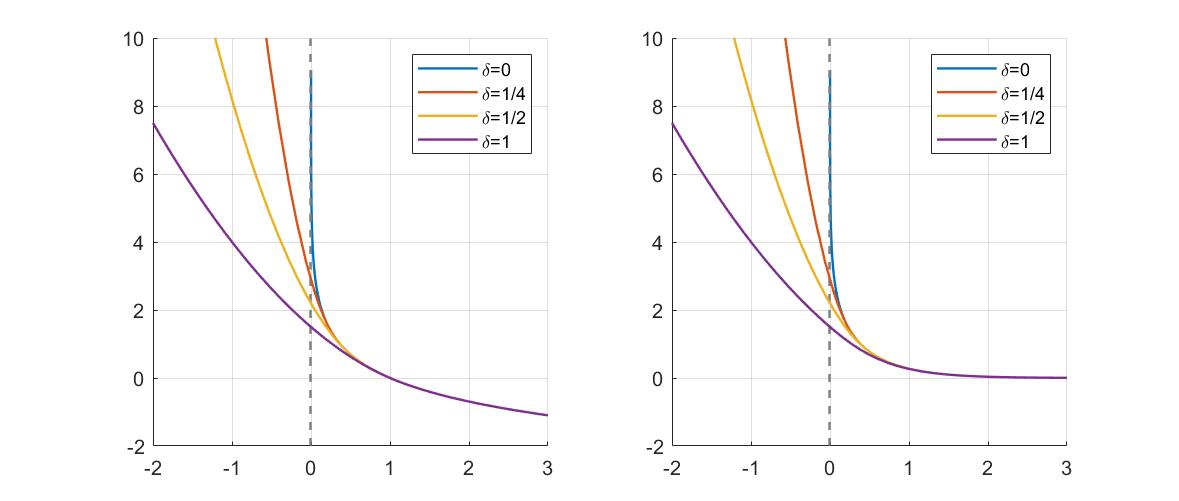
\includegraphics[width=0.8\textwidth]{Images/logbarrierfunc.jpg}
\caption{log barrier functional without (left) and with (right) the hockey stick function}
\label{fig:logbarrierfunc}
\end{figure}

\section{Inter-Vehicular Constraints}
\label{sec:mindistintveh}

\par There are 2 ways of preventing inter-vehicle collision; \textit{spatial deconfliction} and \textit{temporal deconfliction} \cite{hausler2015mission}.
Spatial deconfliction is appropriate for \ac{PF} and imposes the constraint that the spatial paths of the vehicles under consideration will never intersect and keep a desired safe distance from each other. Temporal deconfliction is appropriate for \ac{TT} and requires that two vehicles will never be ”at the same place at the same time”. However, their spatial paths are allowed to intersect. Figure \ref{fig:deconfliction} illustrates the two types of deconfliction strategies. Temporal deconfliction allows an extra degree of freedom and will intuitively lead to cheaper dynamic costs.

\begin{figure}
    \centering
    \begin{subfigure}[b]{0.45\textwidth}
        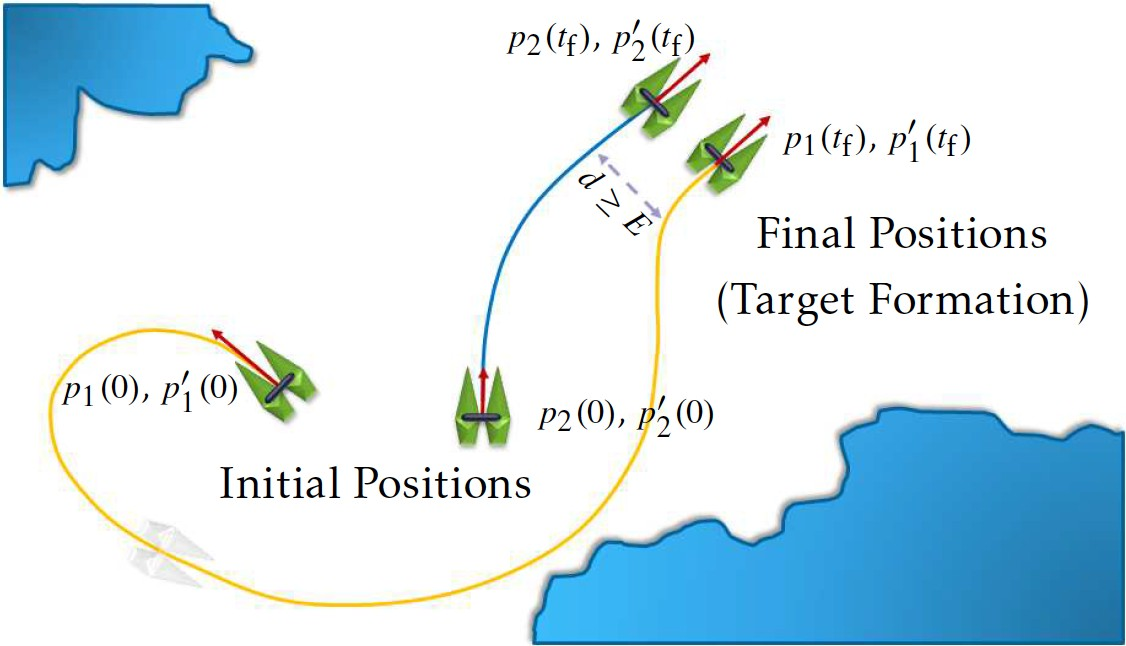
\includegraphics[width=\textwidth]{Images/spacial_deconf.jpg}
        \caption{Spacial Deconfliction}
    \end{subfigure}
    ~
    \begin{subfigure}[b]{0.45\textwidth}
        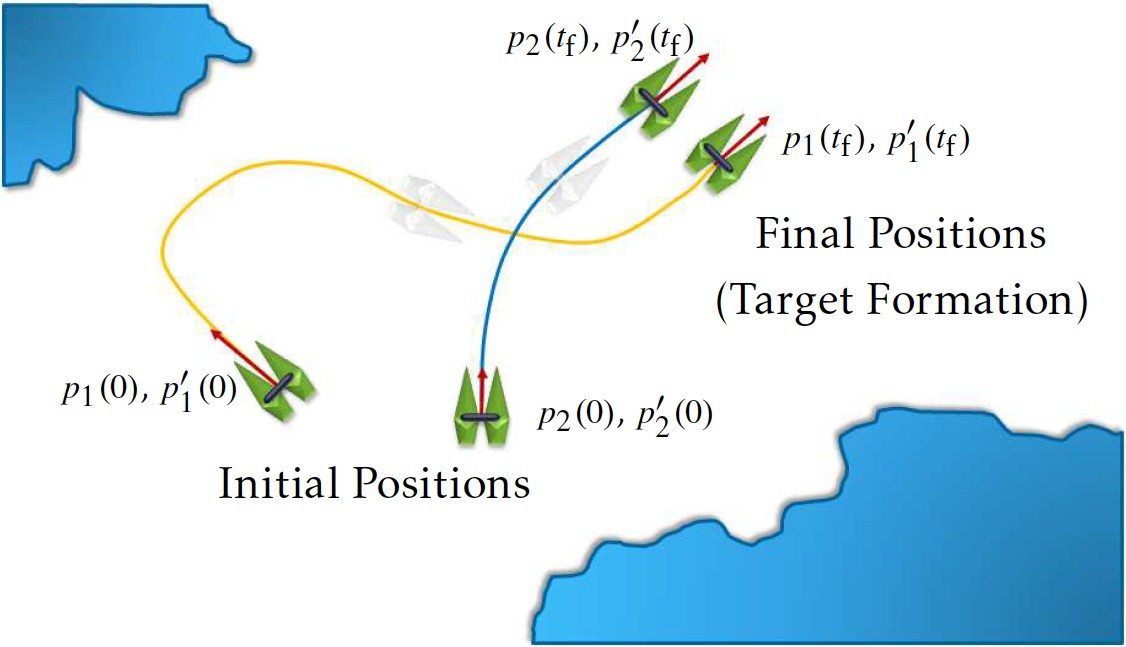
\includegraphics[width=\textwidth]{Images/temporal_deconf.jpg}
        \caption{Temporal Deconfliction}
    \end{subfigure}
    \caption{Inter Vehicle deconfliction Solutions}
    \label{fig:deconfliction}
\end{figure}

\par Two method for temporal deconfliction were implemented, one based on sampling the curves and the other based on directly exploiting the properties of Bezier Curves.

\par For $N_v$ vehicles, any of ${N_v \choose 2}$ pairs could lead to a collision, therefore, all pairs must be tested, which means a quadratic complexity, therefore, finding fast algorithms to calculate the distance between each pair of trajectories becomes essential.
\par The easiest method of guaranteeing that the minimum distance between a pair of vehicles is always above a certain value is by calculating the minimum possible distance between each pair of $N_v$ vehicles, which yields a total of ${N_v \choose 2}$ calculations. If \ac{PF} is used, then the minimum distance between the paths must be created than a certain value. As a result, these paths cannot intersect. If \ac{TT} is used, then the minimum distance between vehicles will depend on time $t \in [0 T]$, which means that the trajectories must intersect in space but not in time. 

\subsection{Sampling Trajectories}

\par Given that this thesis will focus on the usage of \ac{TT} and not \ac{PF}, methods to calculate minimum distances throughout time will be discussed, i.e., minimum distance between trajectories.
\par The most straightforward way to calculate the minimum distance between two trajectories is to sample each trajectory and calculate the euclidean distance between time equivalent samples. The smallest yields the shortest distance. This method, however, is not perfect because the finer the samples, the more accurate is the result. 
\par One thing to note, however, is that super accurate results of minimum distance between trajectories are not necessary. If, besides knowing the position of the vehicle at a sample, we also know the maximum tangent speed between that sample and the next, then the distance to the other vehicle cannot deviate more than a certain determinable value between those 2 points. It will be smaller than the calculated distance if the vehicles are moving towards each other. The choice of number of samples will determine how big this deviation can be. The optimisation algorithm will stop once it finds a minimum distance that is greater than a certain value, therefore, the number of samples must be big enough such that the deviation is relatively small when compared to the desired minimum distance. 
\par For example, an optimisation problem specifies a minimum distance between 2 vehicles of \SI{1}{\meter}. These vehicles are limited to \SI{1}{\meter\per\second}. At a certain point in time between 2 samples, they can be closer to each other than they are at the samples, so lets assume the worst case scenario: half of the time between samples is spent moving towards each other at maximum speed, which implies moving away from each other during the other half of time at maximum speed, therefore, if the time sample is \SI{10}{\milli\second}, during \SI{5}{\milli\second} the vehicles can travel \SI{1}{\centi\meter} towards each other, at the relative speed of \SI{2}{\meter\per\second}, which is a \SI{1}{\percent} deviation from the established minimum distance of \SI{1}{\meter}. If the optimisation problem is reformulated to guarantee \SI{1.01}{\meter}, then, with samples spaced by \SI{10}{\milli\second}, a successful optimisation solution guarantees a minimum distance between vehicles of \SI{1}{\meter}. which means a total of 100 samples per second of runtime.


\subsection{Bezier Curve Distance to a Point}
\label{sec:bezcurvetopoint}

\par The next method is based on calculating the minimum distance between Bezier curves \cite{chang2011computation}. This algorithm is adapted to calculate the minimum distance between a curve and a polygon. By subtracting one trajectory to another, which for Bezier curves is explained in section \ref{sec:bezcurves}, finding the minimum distance between trajectories gets translated to finding the closest point of this subtraction curve to the origin. The origin can be interpreted as a 1 point convex shape, therefore, what follows is a brief explanation of an iterative algorithm to calculate the minimum distance of a Bezier curve to a polygon, which will also be used to do collision avoidance with arbitrary convex shapes.

\par This algorithm consists in recursively breaking down the trajectory into halves by obtaining a new set of control point for each half via de De Casteljau algorithm. For each half, two values are calculated: an upper bound of the minimum distance and a lower bound. The upper bound for the minimum distance will be the closest endpoint of the segment to the polygon, a lower bound is the closest point of the convex hull of the new control points to the polygon. The exit condition of the recursion is when the lower bound is relatively small when compared to the upper bound. The lower bound may be zero if the shapes intersect, which has no influence on the execution of the algorithm. If the exit condition isn't met, the recursion is repeated and the returned value is the smallest of the upper bound along with the time at which the smallest value was found.

\subsection{GJK Algorithm}
\label{sec:gjkalg}

\par The \ac{GJK} algorithm is a necessary tool for calculating the minimum distance between a Bezier Cuve and a point or polygon, therefore, it is explained here.

\par The \ac{GJK} algorithm is an efficient algorithm to calculate minimum distance between arbitrary convex shapes in any dimension. 
\par The \ac{GJK} algorithm relies heavily on a concept called the Minkowski Sum, but, because the difference operator is used for this algorithm, instead of the sum, the term Minkowski difference will be used. For two shapes $A$ and $B$, their Minkowski Difference is given by
\begin{equation}
    D = A - B = \{a-b|a\in A, b\in B\}
\end{equation}
where $D$ is a new convex shape given by the subtraction of every point in $A$ by every point in $B$.
Figure \ref{fig:intersectingshapes} shows 2 shapes on the left hand-side which intersect and the resulting Minkowski Difference on the right hand side. Figure \ref{fig:nonintersectingshapes} shows two shapes that do not intersect and their resulting Minkowski Difference. Notice how the second Minkowski Difference has an identical shape to the first, only differing on its position.
\begin{figure}
\centering
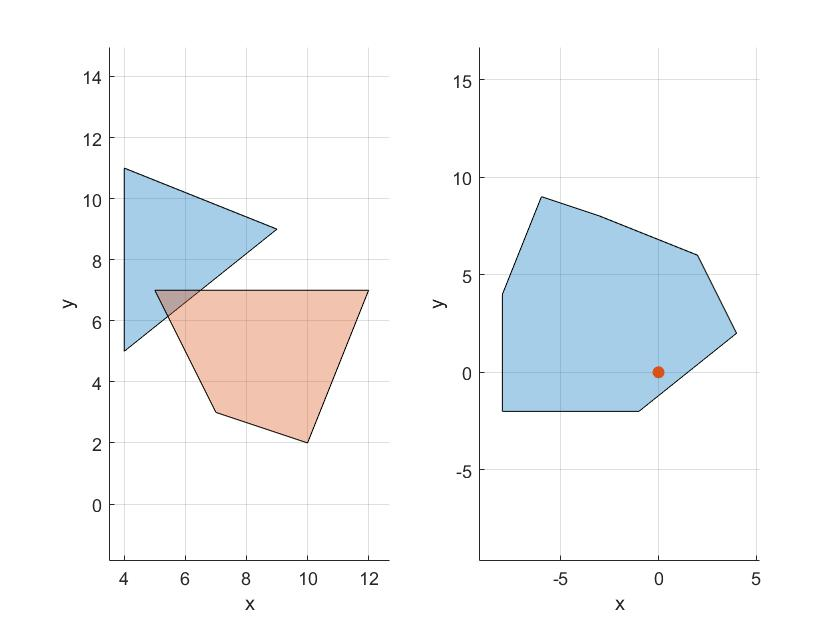
\includegraphics[width=0.8\textwidth]{Images/intersectingshapes.jpg}
\caption{Intersecting convex shapes (left) and resulting Minkowsky Difference (right)}
\label{fig:intersectingshapes}
\end{figure}
\begin{figure}
\centering
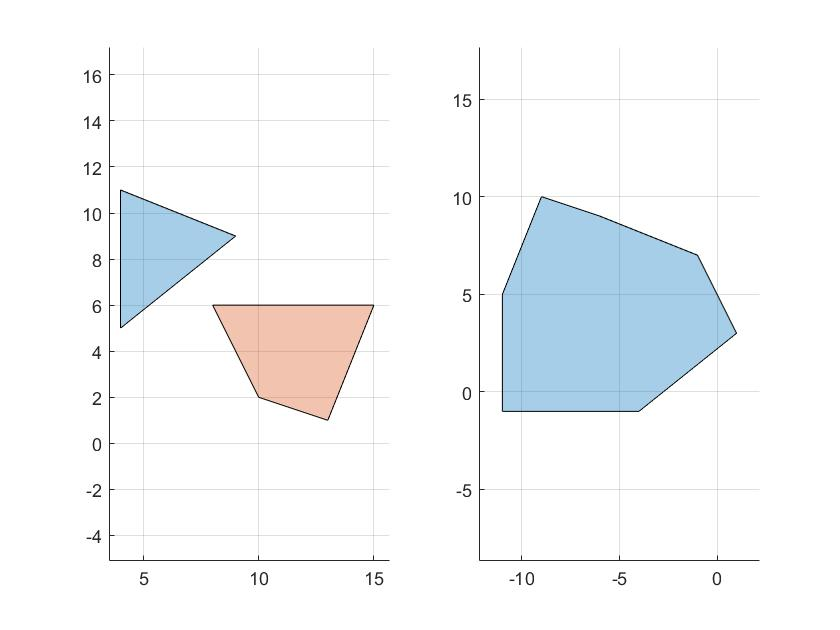
\includegraphics[width=0.8\textwidth]{Images/nonintersectingshapes.jpg}
\caption{Non-intersecting convex shapes (left) and resulting Minkowsky Difference (right)}
\label{fig:nonintersectingshapes}
\end{figure}

\par If the Minkowski Difference contains the origin, then the two shapes have common points, i.e., intersect, because the resulting subtraction is zero. As a result, the \ac{GJK} algorithm is a two part problem: first detect intersection, by testing if the Minkowski Difference contains the origin, then, if it does not, the closest points between $A$ and $B$ result in a Minkowski Point that is closest to the origin, therefore, the second part part of the problem is to look for that closest point to the origin.
\par For a N-D Minkowski Difference, if a convex shape of up to N+1 vertices that surrounds the origin is found, then the shapes $A$ and $B$ intersect. This shape with up to N+1 vertices is known as a simplex. For 2-D Minkowski Differences, the simplexes can be a point (1 vertex), a line segment (2 vertices) and a triangle (3 vertices). For 3-D spaces, the simplexes can be the same as in 2-D spaces with the addition of a tetrahedron (4 vertices).
\par The key to \ac{GJK}'s efficiency is to find points in the Minkowski difference that are the best candidates to be in a simplex that can contain the origin. 
\par A support function returns the farthest point in some direction. The resulting point is known as the support point. Finding a support point in the Minkowski Difference along direction $d$ is the same as subtracting the support point of $A$ along $d$ and $B$ along $d$. 
\par Choosing the farthest point in a direction has significance because it creates a simplex who contains a maximum area therefore increasing the chance that the algorithm exits quickly. In addition, all the points returned this way are on the edge of the Minkowski Difference and therefore if a point past the origin along some direction cannot be added, the Minkowski Difference cannot contain the origin. This increases the chances of the algorithm exiting quickly in non-intersection cases.

\par Let $W_k$ be the set of vertices of the simplex constructed in the $k^{th}$ iteration, and $v_k$ as the point in the simplex closest to the origin. Initially, $W_0=\varnothing$, and $v_0$ is an arbitrary point of the Minkowski Difference. Since each $v_k$ is contained in the Minkowski Difference, the length of $v_k$ must be an upper bound for the distance.
\par \ac{GJK} generates a sequence of simplices in the following way. In each iteration step, a vertex $w_k = s_{A-B}(-v_k)$ is added to the simplex, with the objective of surrounding the origin. If the simplex contains the origin, then the program interrupts because the shapes intersect. If it's proven that the Minkowski Difference cannot contain the origin because the last added vertex did not move "beyond" the origin, then program interrupts and moves on to finding the minimum distance to the origin. If intersection is not proven yet, the new $v_{k+1}$ is perpendicular to the vector given by the last vertex with the one before that, or with the last with the third from the last, if available, depending on which has a dot product greater than 0, and the not used vertex gets removed from the simplex. Alternatively, if no intersection is proven, the new $v_{k+1}$ is the point in the convex hull of $W_k\cup \{w_k\}$ closest to the origin and $W_{k+1}$ becomes the smallest sub-simplex of $W_k\cup \{w_k\}$ that contains $v_{k+1}$.


\section{Minimum Distance to Convex Shapes}
\label{sev:mindistconvshapes}

\par Earlier, in section \ref{sec:bezcurvetopoint}, an algorithm to calculate the distance of a trajectory to a polygon was presented. This algorithm, however, is limited to polygons that do not intersect with the trajectory. If the curve intersects with the convex shape, the algorithm returns zero as minimum distance. Optimisation algorithms, like Sequential Quadratic Programming, require the derivative of the constraints to be non zero, even when the current guess for solution is not feasible because this derivate, in other words, will "inform" how far the control points must move so that the solution becomes feasible.

\par A modification to the algorithm that calculates the minimum distance to a convex shape is presented to calculate the intersection points between the curve and the shape. Afterwards, these intersection points are used to calculate a "penetration" of the curve in the shape.
\par First thing to note is, during the recursion of the minimum distance algorithm, some endpoints of the cut segments will land inside the shape. If a segment has an endpoint inside and an endpoint outside the shape and the distance between these two points is approximately zero, then the point inside is added to a stack of intersecting points, otherwise, the recursion continues. If the control points of the recursive segments are partially in the shape while others are not, then the recursion continues, otherwise, if the control points are all outside or all inside the shape, then there is no point in continuing because the segment cannot contain any more intersection points.
% \par One thing that can be pointed out that can speed up checking if all of the control points of a segment are contained in the shape or not is by finding the convex hull of of the shape. If some control points are on the convex hull. The advantage of this way of testing if all control points are in the shape is that the complexity of the convex hull algorithm, will be $\mathcal{O}(n\log{}n)$, 
\par Once the intersection points are found, the "penetration" must be calculated. This consists first in finding a convex hull that intersects the shapes. If the number of intersection points is two, then the De Casteljau algorithm is performed twice to find a set of control points for the segment that starts and ends with these two points and the convex hull of these control points is taken, otherwise, the convex hull of all of the intersecting points is used. Once the convex hull is determined, the \ac{DEPA} algorithm explained in section \ref{sec:epaalg}  is performed with the obstacle shape along a predefined direction $d$. The bigger the penetration depth, the more the trajectory is "deeper" in the curve.



\subsection{Directed EPA}
\label{sec:epaalg}

% https://graphics.stanford.edu/courses/cs468-01-fall/Papers/van-den-bergen.pdf

\par If two convex shapes intersect, the \ac{GJK} algorithm cannot provide collision information like the penetration depth and vector. One algorithm that provides this information is the \ac{EPA}.
A slight modification for the \ac{EPA} algorithm is proposed here. It will be referred as the \ac{DEPA}, whose objective is to find the penetration of one convex shape relative to another along a specific direction $d$, while the \ac{EPA} algorithm finds the shortest vector such that the shapes no longer collide. The penetration along a direction is the length of dislocation that the second shape would have to move so that the two shapes no longer collide. 
\par The shapes intersect when the Minkowski contains the origin, therefore, the \ac{EPA} or the slight variant shown here have as objective dislocating the Minkowski Difference such that it no longer contains the origin. Penetration along a specific direction can be found by calculating the length of the vector that starts in the origin on the Minkowski Difference, has the same direction as $d$, and stops once it finds the edge of the Minkowski Difference. In other words, this is the norm of the intersection point between a ray starting at the origin with direction $d$ and the edge of the Minkowski Difference. Once this length is found, shape $B$ can move by that length along the direction of $d$ such that it is no longer in collision with shape $A$.
\par The process of looking for the penetration along a direction $d$ starts with a polygon which contains the origin, constructed with points along the edge of the Difference. The first step is to find the only edge of this polygon with will intersect with the ray that starts in the origin with direction $d$. Once this edge is found, the other edges of the polygon are ignored and an iterative process starts. The first step on the iterative process is to calculate a vector which normal to the current intersecting segment and points "outwards" with respect to the origin. Next, the support function is performed with this vector. The resulting point will be closer to the desired final point. There are now three points in play: the two segment ends and the new point that resulted from the support operation. The next step is to define two segments, one from the one of the segment ends to the new support point, the other from the other segment end to the support point. The next step is to find which of these two new segments intersects with the same ray with direction $d$ and then repeat the iteration. 



\section{Description of the implemented code}
\label{sec:description_implementation}

\par The variables for the motion planning problem are each vehicle's state variables and inputs, as explained in section \label{sec:theoptproblem}. Each of these variables will be referred to as curves. Optimisation algorithms cannot take continuous functions as variables, therefore, some form of parameterisation of each curve is necessary, as exemplified in some of the algorithms of chapter \label{chap:theory}. Here, each curve will be represented as a Bernstein Polynomial with order $N$, which will require $N+1$ control points. A distinction is made between state variables and inputs: state variables must have established initial and final conditions, inputs do not. This implies that for state variables, the initial and final control points must be fixed, therefore, they do not need to participate on the optimisation problem. The following matrix represents how the control points are stored so that they can be accessed by all functions that perform operations on the curves.

\begin{equation}
    \begin{bmatrix}
        \colorbox{yellow}{$\displaystyle x_0^0$} & \colorbox{yellow}{$\displaystyle y_0^0$} & \colorbox{yellow}{$\displaystyle \psi_0^0$} & \colorbox{yellow}{$\displaystyle u_0^0$} & \colorbox{yellow}{$\displaystyle v_0^0$} & \colorbox{yellow}{$\displaystyle r_0^0$} & \tau_{u_0}^0 & \tau_{r_0}^0 \\
        x_1^0 & y_1^0 & \psi_1^0 & u_1^0 & v_1^0 & r_1^0 & \tau_{u_1}^0 & \tau_{r_1}^0 \\
        \vdots & \vdots & \vdots & \vdots & \vdots & \vdots & \vdots & \vdots \\
        \colorbox{yellow}{$x_{N}^0$} & \colorbox{yellow}{$y_{N}^0$} & \colorbox{yellow}{$\psi_{N}^0$} & \colorbox{yellow}{$u_{N}^0$} & \colorbox{yellow}{$v_{N}^0$} & \colorbox{yellow}{$r_{N}^0$} & \tau_{u_{N}}^0 & \tau_{r_{N}}^0
    \end{bmatrix}
    \label{eq:matrixofvariables}
\end{equation}

\par It is believed \todo{can this be said? because I'm not referencing anything (I'm taking Venanzio's word for it)} that \texttt{fmincon()} performs better when all variables are stored in a line vector, therefore, a function called \texttt{matrify()} is necessary in order to transform the flattened optimisation variable to the matrix of equation (\ref{eq:matrixofvariables}). 
\par Elements marked in yellow do not participate in the optimisation algorithm. They are concatenated to this matrix in \texttt{matrify()}. 

\par High orders are preferable for each curve \cite{cichella2018bernstein} because the higher the curve, the closer the control points are to the "matching" point in time of the curve, which is achieved once an optimisation problem finishes. Chapter \ref{chap:results} exemplifies show the control points approximate to the curve and how it is advantageous to produce the dynamics.

%\par A more precise way to calculate the minimum distance of a Bezier curve to a point or to another curve, compared to the one implemented on section \ref{sec:2_d_bezier} is via the algorithm presented in \cite{chang2011computation}. This algorithm takes into account the convex hull property of Bezier Curves and the \textit{deCasteljau} algorithm for subdividing curves. It will also employ the GJK algorithm, a fast and efficient way of calculating distances between 2 convex shapes\cite{cichella2018bernstein}.
%\par The fast calculation of distances between these curves allows Bezeir Curves to be appropriate for testing non-linear constraints in multiple vehicle motion planning optimisation.
%
%\par This fancy algorithm performed poorly because it was iterative. A simpler way to calculate the minimum distance was necessary. This consited in subtracting each pair of 2-D curves for each vehicle to eachother, then getting a rough guess of the closest point of that resulting curve to 0: by performing degree elevation to an order 10 times the original then looking for the closest point to the origin. 
%
%\par Minimum distance of the curves to objects was done with GJK. but it was slow
%
%\par Collision to circles is calculated by subtracting the 2-D curve tto the centre of the circle, performing degree elevation of the resultign curve, calculating the closest to the origin and checking wether that distance is greater to the radius. Performing the check for every control point was also done but wasn't advantageous (slower runtime), the reason could be because the derivative of each of these distances or the elevated curve with respect to the position of the control points depends on more than 1 control points of the non elevated curve, therefor, some computation is redundant.


\par The optimisation problem is formulated by constructing a data structure with the fields of table \ref{tab:constants_description}. %In Python the same fields are necessary, however, they must be stored in a python dictonary. 


\begin{table}[]
\centering
\begin{tabular}{|l|l|l|l|}
\hline
\textbf{field} & \textbf{description} & \textbf{mandatory} & \textbf{example} \\ \hline
\texttt{T} & Time horizon & yes & \texttt{10} \\ \hline
\texttt{xi} & initial conditions & yes & \texttt{[0 0 0 1 0]} \\ \hline
\texttt{xf} & final conditions & yes & \texttt{[5 5 pi/2 1 0]} \\ \hline
\texttt{N} & order of the curves & yes & \texttt{15} \\ \hline
\texttt{obstacles} & polygons & \begin{tabular}[c]{@{}l@{}}no\\ default: \texttt{[]}\end{tabular} &  \\ \hline
\texttt{obstacles\_circles} & circles & \begin{tabular}[c]{@{}l@{}}no\\ default: \texttt{[]}\end{tabular} &  \\ \hline
\texttt{min\_dist\_int\_veh} & \begin{tabular}[c]{@{}l@{}}minimum distance between \\ vehicles for every point in time\end{tabular} & \begin{tabular}[c]{@{}l@{}}no\\ default: \texttt{0}\end{tabular} & \texttt{.8} \\ \hline
\texttt{numinputs} & \begin{tabular}[c]{@{}l@{}}number of input variables\\ (don't have initial conditions)\end{tabular} & \begin{tabular}[c]{@{}l@{}}no\\ default: \texttt{0}\end{tabular} &  \\ \hline
\texttt{uselogbar} & \begin{tabular}[c]{@{}l@{}}make the problem completely \\ unconstrained and use log \\ barrier functionals\end{tabular} & \begin{tabular}[c]{@{}l@{}}no\\ default: \texttt{false}\end{tabular} &  \\ \hline
\texttt{usesigma} & \begin{tabular}[c]{@{}l@{}}a boolean for the usage of the \\ sigma function if log barrier \\ functionals are to be used\end{tabular} & \begin{tabular}[c]{@{}l@{}}no\\ default: \texttt{false}\end{tabular} &  \\ \hline
\texttt{costfun\_single} & \begin{tabular}[c]{@{}l@{}}a function used to calculate \\ the running cost for each \\ singular vehicle\end{tabular} & yes & \texttt{@costfun} \\ \hline
\texttt{dynamics} & \begin{tabular}[c]{@{}l@{}}a function that describes how the \\ non linear dynamics of the state \\ variables and inputs are linked\end{tabular} & yes & \texttt{@dynamics} \\ \hline
\texttt{init\_guess} & \begin{tabular}[c]{@{}l@{}}a function that provides an initial \\ guess for the optimisation problem \\ which may  speed up the process \\ of optimisation\end{tabular} & \begin{tabular}[c]{@{}l@{}}no \\ default:\\ \texttt{@rand\_init\_guess}\end{tabular} & \texttt{@init\_guess} \\ \hline
\texttt{recoverxy} & \begin{tabular}[c]{@{}l@{}}a function that returns the x and y\\ variables by solving just the initial \\ value problem of the inputs\end{tabular} & yes & \texttt{@recoverxy} \\ \hline
\end{tabular}
\caption{Description of the constants for optimisation}
\label{tab:constants_description}
\end{table}


\par Some notes for each of the fields:

\begin{itemize}
    \item \texttt{xi} has as many lines as state variables (not input variables) and as many lines as number of vehicles. Because these functions are designed for vehicles, $x$ and $y$ must be in the first 2 columns
    \item \texttt{xf} works just as \texttt{xi}
    \item \texttt{obstacles\_circles}  Ncircles by 3, where columns are x, y and radius, respectively
    \item \texttt{recoverxy} takes an aribtrary $X$ matrix and and a \texttt{constants} structure and returns a Npoints by 2 matrix
    \item \texttt{dynamics} takes in an arbitrary X matrix and constants structure (to provide pre computer information like a derivation matrix) and must return a column vector which is zeros when all of the dynamic constraints are respected
\end{itemize}

\par The data structure for the nonlinear optimisation problem is then passed to a function called \texttt{run\_problem} which returns the control points for each of the defined variable along with computation time.

\subsection{Dynamics}
\label{sec:dynamics}

\par The dynamics are guaranteed with the formulation of \ref{eq:multi_cost_bern}. This means that the code version for the dynamics plus kinematics for the Medusa vehicle, for example, which are  \ref{eq:simple_medusa_kinematics} and \ref{eq:simple_medusa_dynamics}, become

\begin{lstlisting}[language=matlabfloz,caption={\mcode{Matlab Function}}]
ceq = [
    DiffMat*x - u.*cos(yaw) + v.*sin(yaw) - Vcx;
    DiffMat*y - u.*sin(yaw) - v.*cos(yaw) - Vcy;
    DiffMat*yaw - r;
    DiffMat*u - 1/m_u*(tau_u + m_v*v.*r - d_u.*u+fu);
    DiffMat*v - 1/m_v*(-m_u*u.*r - d_v.*v+fv);
    DiffMat*r - 1/m_r*(tau_r + m_uv*u.*v - d_r.*r+fr);
];
\end{lstlisting}

\par As explained in section \ref{sec:theoptproblem}, \texttt{Diffmat} preserves the order and the equality is maintained in the control points, not the values of the curve itself so some approximation error is expected, which can be minimized with higher orders.

\par Given that each variable is defined by a set of control points, and, using the convex hull property of Bernstein polynomials, upper and lower bounds for each variable, state or input, become the biggest or smallest control point, respectively.

\section{Check Soundness with IVP Solution}
\label{sec:ivproblem}

\par Once the optimisation process gets completed, the trajectory is defined along with, depending on the used model, the control points for the inputs which can then be re-plugged into the \ac{ODE} and check what resulting trajectory is obtained, this process is known as solving an \ac{IVP}. If the approximation is good enough, the resulting trajectory should be nearly identical to the the function for the trajectory. 


% If Printing on DOUBLE SIDED pages, the second page should be white.
% Otherwise, comment the following command:
\cleardoublepage
%
%Chapter 5
% #############################################################################
% This is Chapter 5
% !TEX root = ../main.tex
% #############################################################################
% Change the Name of the Chapter i the following line
\fancychapter{Results}
\cleardoublepage
% The following line allows to ref this chapter
\label{chap:results}

\par The following results are based on solving the optimisation problem \eqref{eq:multi_cost_bern} with the implementation described in section \ref{sec:description_implementation}.
\par Sequential Quadratic Programming \cite{10.1007/978-0-387-35514-6_7} will be the nonlinear programming solver of choice. Simulations were run on a 4 × Intel\textsuperscript{\textcopyright} Core\texttrademark i5-7200U CPU @ 2.50GHz processor. 


\par Several different running cost functions were tested such as 
\begin{equation}
    J = \int_0^T \frac{du}{dt}^2 dt
\end{equation}
which minimizes tangent acceleration,
\begin{equation}
    J = \int_0^T u^2 dt
\end{equation}
which minimizes speed, and finally, for the Medusa model, specifically,
\begin{equation}
    J = \int_0^T \tau_u^2 + \tau_r^2
\end{equation}
which minimizes the input.
\par All of these serve as proxies to the minimisation of spent energy.

\par Results for the two models presented in chapter \ref{chap:autonomousvehiclemodels} are presented. The unicycle model has a total of 5 state variables while the Medusa model has a total of 6 state variables plus 2 inputs. Upper and lower bounds for each variable for each vehicle were implemented as explained in section \ref{sec:dynamics}, by finding the biggest and smallest control points. For the examples presented in this chapter, the bounds that were used are those presented in table \ref{tab:variablebounds} which were chosen to closer represent a real Medusa vehicle.
\begin{table}[h!]
\centering
\begin{tabular}{|l|l|l|l|}
\hline
& Variable & Starting Conditions & Final Conditions \\ \hline
Dubin's Car & $x$ & $-\infty$ & $\infty$ \\
& $y$ & $-\infty$ & $\infty$ \\
& $\psi$ & $-\infty$ & $\infty$ \\
& $u$ & 0 & 1.1 \\
& $r$ & $-\pi/4$ & $\pi/4$ \\ \hline
Medusa & $x$ & $-\infty$ & $\infty$ \\
& $y$ & $-\infty$ & $\infty$ \\
& $\psi$ & $-\infty$ & $\infty$ \\
& $u$ & 0 & 1.1 \\
& $v$ & $-\infty$ & $\infty$ \\
& $r$ & $-.74$ & $.74$ \\
& $\tau_u$ & 0 & 25.9 \\
& $\tau_r$ & -.113 & .113 \\
\hline
\end{tabular}
\caption{Upper and lower bounds for each variable of each vehicle model}
\label{tab:variablebounds}
\end{table}

\par A significant number of experiments were performed to the optimisation algorithm in order to study its behaviour with changing parameters. Out of all of the experiments that were performed, the most relevant will be presented.

\section{No obstacles}

\par The first problem will be run for both a single Dubin's car and a single Medusa vehicle, with initial and final states described in table \ref{tab:firstproblem} and no obstacles. Figures \ref{fig:noobstaclesfigures} and \ref{fig:noobstaclesmedusa} show solutions for order 20 and a time horizon of . Each example has a different combination of vehicle model and cost function. Both models contain control points to describe $x$ and $y$ positions, which is what the blue lines show. The red lines describe the solution of the Initial Value Problem as described in section \ref{sec:ivproblem}. This figure, and all that remain, flip x and y axis which standard for marine vehicles.

\begin{table}[h!]
\centering
\begin{tabular}{|l|l|l|}
\hline
Variable & Starting Conditions & Final Conditions \\ \hline
$x$ & 0 & 30 \\
$y$ & 0 & 30 \\
$\psi$ & 0 & $\pi/2$ \\
$u$ & 1 & 1 \\
$v$ & 0 & 0 \\
$\omega$ & 0 & 0 \\
\hline
\end{tabular}
\caption{Initial and final conditions for a basic Motion Problem}
\label{tab:firstproblem}
\end{table}


\begin{figure}[h!]
\centering
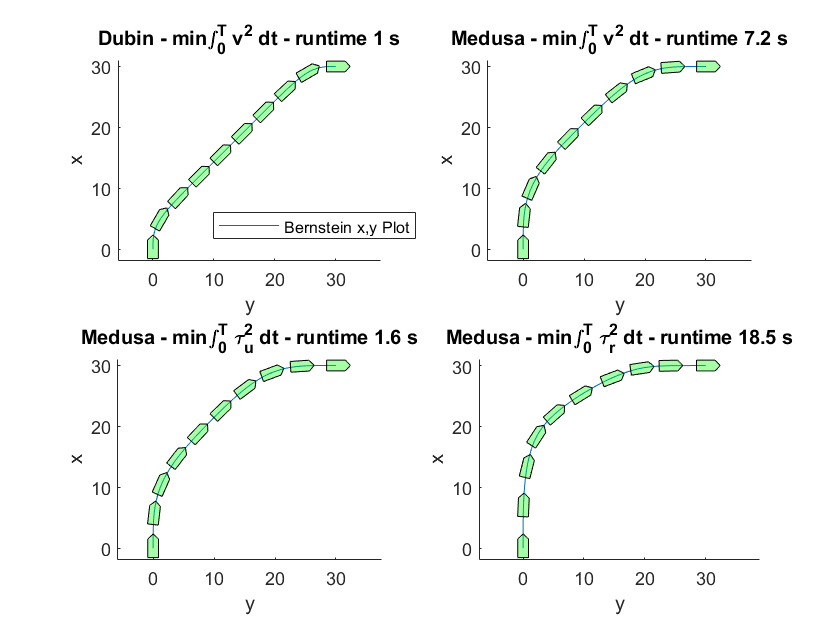
\includegraphics[width=0.8\textwidth]{Images/results/noostaclesfigures.png}
\caption{Solutions of order $N=20$ without obstacles and final time $T=60$}
\label{fig:noobstaclesfigures}
\end{figure}

\begin{figure}[h!]
\centering
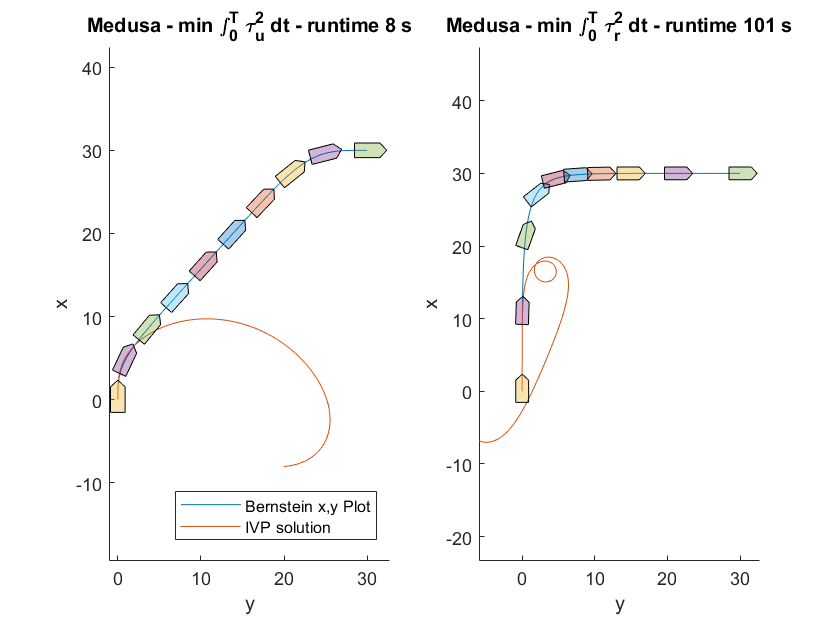
\includegraphics[width=0.8\textwidth]{Images/results/noostaclesmedusa.png}
\caption{Solutions of order $N=20$ that minimize $\tau_u^2$ (left) and $\tau_r^2$ (right) for the Medusa Model with time horizon $T=60$}
\label{fig:noobstaclesmedusa}
\end{figure}

\par First thing to note is, despite all executions running successfully, i. e., the optimal and feasible solution was found, the Medusa's \ac{IVP} solution resembles less the plot of the Bezier curve of the x and y control points when compared with the Dubin's car. This suggests that the order isn't high enough for the curves to accurately represent the real optimal solution's state variables for the Medusa model, which is more complex. 


\section{Obstacles}

\par The following figures show solutions with circle or polygon obstacles whose collision avoidance algorithms are explained in sections \ref{sec:mindistintveh} and \ref{sec:mindistconvshapes}. Figure \ref{fig:baselineresult} is the baseline example without obstacles. It uses a Dubin's Car with the same initial and final conditions as in the previous section and minimises $v^2$. Figure \ref{fig:circleobstacle}, shows the solution with the added circle as a constraint. Figure \ref{fig:circleobstaclelogbargood} shows the solution with an obstacle but the constraint was moved to the log barrier functional as explained in section \ref{sec:logbarrierfunc}. Figure \ref{fig:circleobstaclelogbarbad} shows the solution with log barrier funcitonal as well but the relative weight of the log barrier on the cost wasn't as big, and, as a result, the optimisation problem terminated successfully but did not prevent collision. The runtimes of these examples don't show how the usage of log barrier provides an advantage, however, for a polygon obstacle, such as in figures \ref{fig:polygonobstacle} and \ref{fig:polygonobstaclelogbar} show a huge difference in the usage of the log barrier functional. Both these results have a huge runtime when compared to circular obstacles because the algorithm is iterative.

\begin{figure}[h!]
\centering
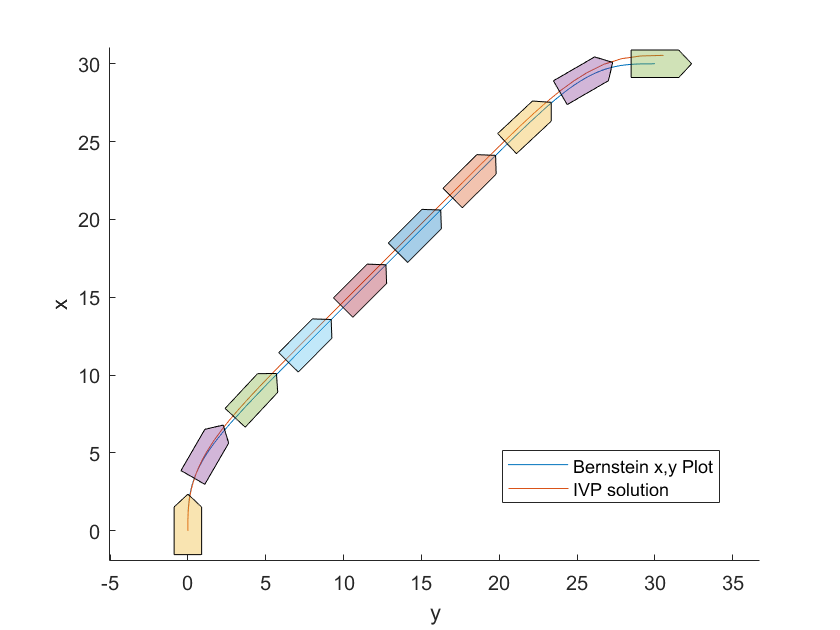
\includegraphics[width=0.8\textwidth]{Images/results/baselineresult.png}
\caption{Solution of order $N=20$ without obstacles \\ computation time = 2s}
\label{fig:baselineresult}
\end{figure}

\begin{figure}[h!]
\centering
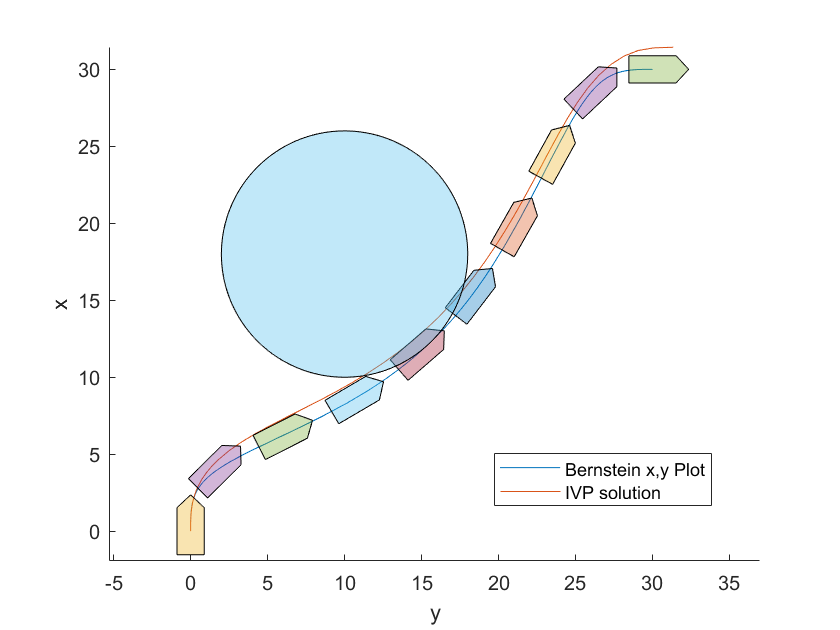
\includegraphics[width=0.8\textwidth]{Images/results/circleobstacle.png}
\caption{Circle osbtacle: computation time 5s}
\label{fig:circleobstacle}
\end{figure}

\begin{figure}[h!]
\centering
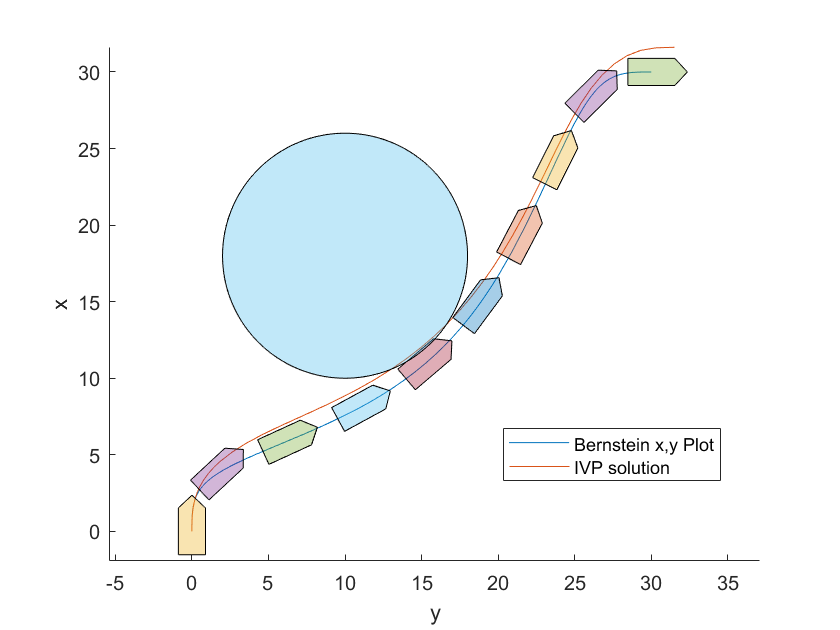
\includegraphics[width=0.8\textwidth]{Images/results/circleobstaclelogbargood.png}
\caption{Circle obstacle plus log bar: computation time 4s}
\label{fig:circleobstaclelogbargood}
\end{figure}

\begin{figure}[h!]
\centering
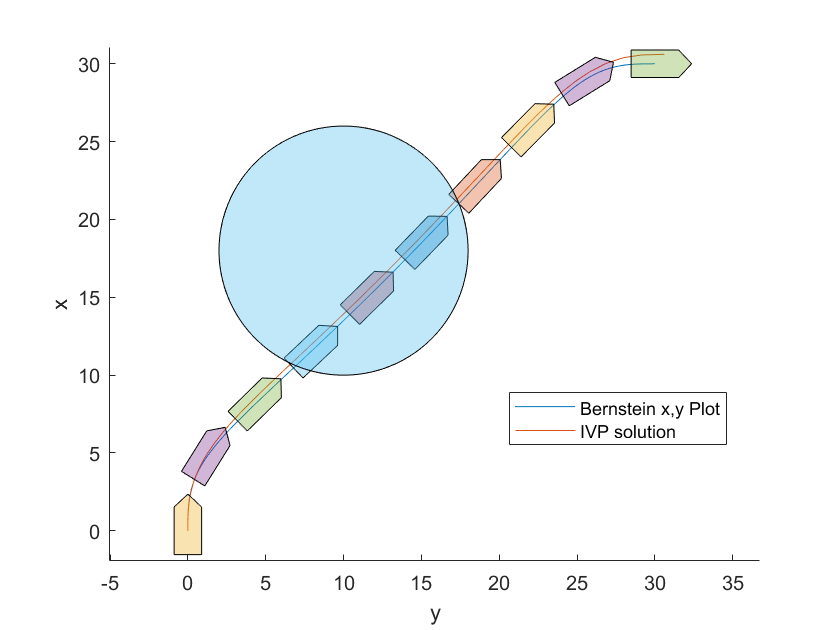
\includegraphics[width=0.8\textwidth]{Images/results/circleobstaclelogbarbad.png}
\caption{Circle obstacle plus log bar: computation time 3s}
\label{fig:circleobstaclelogbarbad}
\end{figure}

\begin{figure}[h!]
\centering
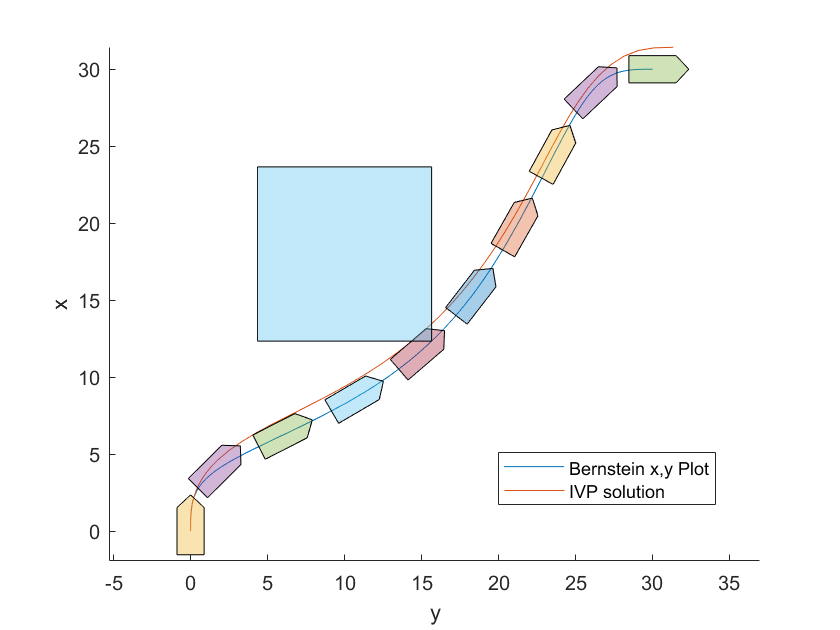
\includegraphics[width=0.8\textwidth]{Images/results/polygonobstacle.png}
\caption{polygon obstacle: computation time 307s}
\label{fig:polygonobstacle}
\end{figure}

\begin{figure}[h!]
\centering
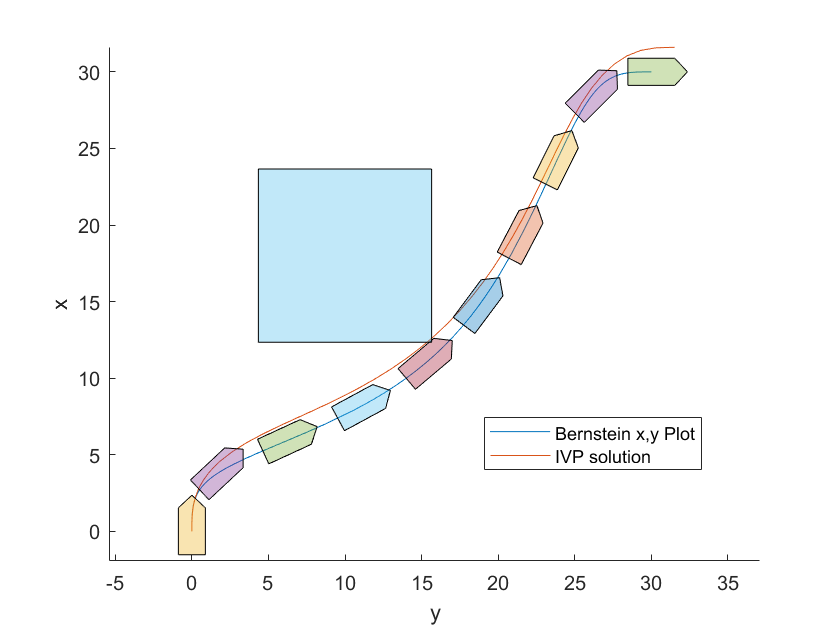
\includegraphics[width=0.8\textwidth]{Images/results/polygonobstaclelogbar.png}
\caption{polygon obstacle: computation time 157s}
\label{fig:polygonobstaclelogbar}
\end{figure}


\subsection{Variation of cost with order}

\par The next step was to implement a way of calculating solutions for high orders while maintaining low computation time. This is acheived by taking the solution of a low order, perform degree elevation and re-feed that solution as initial guess for a higher order. Figure \ref{fig:progressiveNexamples}, show some solutions of this procress. The top left figure started is the solution order 10, this solution has it's order increased by 10, and used as initial guess for another run resulting in the top right figure and so on and so on. The iterative process stopped with order 70 because the relative final cost differs from order 60 by less than 1\%. The same solution of oder 70 took a total of 334 seconds when using a random initial guess which shows how this iterative method can save computation time.

\begin{figure}[h!]
\centering
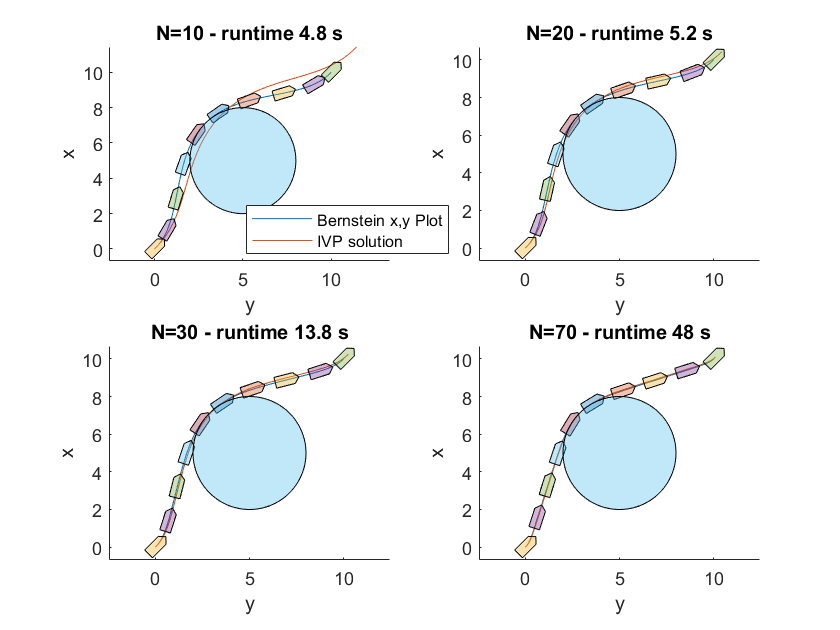
\includegraphics[width=0.8\textwidth]{Images/results/progressiveNexamples.png}
\caption{Results of Interatively increasing order}
\label{fig:progressiveNexamples}
\end{figure}



\par We can see how to cost varies with increase of order $N$ and how the solution of the \ac{IVP} becomes closer and closer to the plot of $xy$.





\section{Multiple Vehicles}

\par In figure \ref{fig:multiplevehicles} we can see how computation time quickly grows with even a small number of vehicles for a Medusa model and using the sampling approach for deconfliction discussed in \ref{sec:mindistintveh}.

\begin{figure}[h!]
\centering
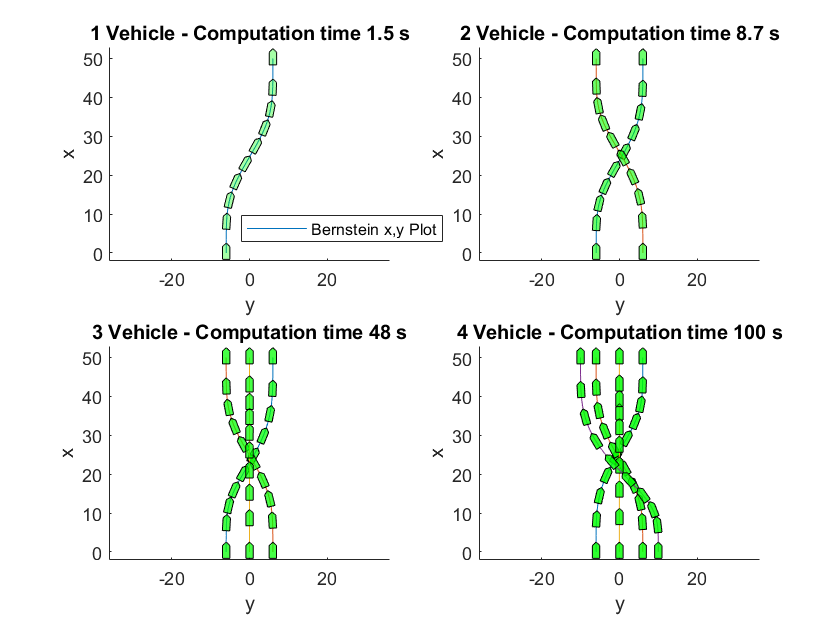
\includegraphics[width=0.8\textwidth]{Images/results/multiplevehicles.png}
\caption{Solutions of order $N=10$ with multiple vehicles}
\label{fig:multiplevehicles}
\end{figure}


\par And at last an example with 3 vehicles and 1 obstacle, in figure \ref{fig:finalexample}

\begin{figure}[h!]
\centering
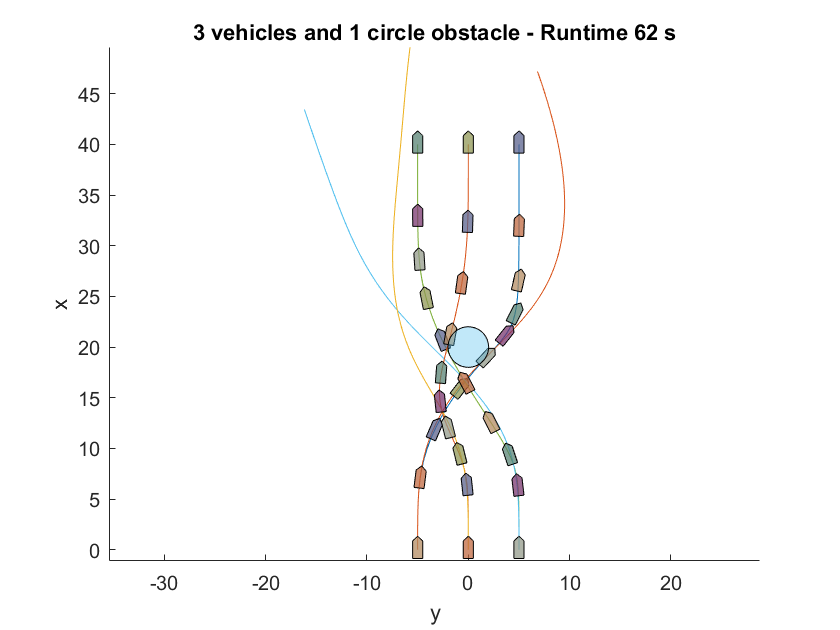
\includegraphics[width=0.8\textwidth]{Images/results/finalexample.png}
\caption{Solution of order $N=10$ with 3 vehicles and 1 circle obstacle}
\label{fig:finalexample}
\end{figure}
% If Printing on DOUBLE SIDED pages, the second page should be white.
% Otherwise, comment the following command:
\cleardoublepage
%
%Chapter 6
% #############################################################################
% This is Chapter 6
% !TEX root = ../main.tex
% #############################################################################
% Change the Name of the Chapter i the following line
\fancychapter{Conclusion}
\cleardoublepage%
\label{chap:conclusion}

% #############################################################################
\par The project was carried out within the master's program Robotics and Control under the supervision of Professor Pascoal. It consisted of the development a fast optimal motion planning algorithm for finding feasible and safe trajectories for a group of vehicles such that they reach a number of target points at the same time. It involed solving an optimal control problem by finding its equivalent finite dimensional optimization problem. The final form of the algorithm was chosen based on the comparison of several parameterization methods and their performance in handling dynamics and environmental constraints. Bezier curves were the final choice of parameterization to approximate the optimal trajectory due to their convenient properties that allow efficient computation and enforcement of constraints along the vehicles’ trajectories.



\par The motion planning algorithm was tested with two \ac{AMV} models: the Dubin's car model and the Medusa model, whose ruling kinematic and dynamics equations were also studied and presented here. It can be concluded that motion planning can now be performed for non-differentially flat systems such as the Medusa model.
\par Results of the application tests show how, with increasing order, the final cost quickly converges to optimal but at the expense of computation time. As a result, a trade-off must be found between optimality and the computation time when deploying the proposed algorithms in real life scenarios. It also can also be concluded that introducing an iterative algorithm in each step of the optimization process - such as the presented \textit{minimum distance to a polygon algorithm} presented here - introduces a disproportionate amount of computation time.
\par A trade off must also be found between order and number of vehicles, because as it has been seen in the tests, the computation time can quickly grow when adding more vehicles, even when the fastest sample-based minimum distance algorithms are used.
\par The motion planning algorithm, not only solves the problem for the go-to-formation maneuver but also supports other kinds of missions such as those based on active navigation. Therefore, future research can be based on applying the algorithms presented here for a wide range of complex motion planning problems. Another further investigation that can be derived from this work is testing the motion planning algorithms in close cooperation with trajectory tracking such that there can be real applied in real time.



%\par In this work, a fast optimal motion planning algorithm was designed. It consisted in solving an optimal control problem, by finding its equivalent finite dimensional optimization problem. The algorithm's final form was chosen based on the comparison of several parameterization methods and how well each one can handle dynamic and environmental constraints. Bezier curves was the final choice of parameterization to approximate the optimal trajectory. They have very good properties for motion planning that greatly simplify the optimization problem.
% If Printing on DOUBLE SIDED pages, the second page should be white.
% Otherwise, comment the following command:
\cleardoublepage%
%
% -----------------------------------------------------------------------------
% BIBLIOGRAPHY
% Add the Bibliography to the PDF table of contents (not the document table of contents)
\pdfbookmark[0]{Bibliography}{bib}
% https://www.overleaf.com/learn/latex/Bibliography_management_with_biblatex
\printbibliography%
% The bibliography style sheet
%% If Printing on DOUBLE SIDED pages, the second page should be white.
%% Otherwise, comment the following command:
\cleardoublepage%

% -----------------------------------------------------------------------------
% HERE GO THE APPENDIXES IF REQUIRED
% If not required just comment the blocks
%\appendix
%% First Appendix
%\pdfbookmark[1]{Appendix A}{appendix}
%% #############################################################################
% This is Appendix A
% !TEX root = ../main.tex
% #############################################################################
\chapter{Code of Project}%
\label{chapter:appendixA}

Nulla dui purus, eleifend vel, consequat non, dictum porta, nulla. Duis ante mi, laoreet ut, commodo eleifend, cursus nec, lorem. Aenean eu est. Etiam imperdiet turpis. Praesent nec augue. Curabitur ligula quam, rutrum id, tempor sed, consequat ac, dui. Vestibulum accumsan eros nec magna. Vestibulum vitae dui. Vestibulum nec ligula et lorem consequat ullamcorper. 


%% If Printing on DOUBLE SIDED pages, the second page should be white.
%% Otherwise, comment the following command:
%\cleardoublepage%
%%% Second Appendix
%\pdfbookmark[1]{Appendix B}{appendix}
%% #############################################################################
% This is Appendix B
% !TEX root = ../main.tex
% #############################################################################
\chapter{A Large Table}
\label{chapter:appendixB}

Aliquam et nisl vel ligula consectetuer suscipit. Morbi euismod enim eget neque. Donec sagittis massa. Vestibulum quis augue sit amet ipsum laoreet pretium. Nulla facilisi. Duis tincidunt, felis et luctus placerat, ipsum libero vestibulum sem, vitae elementum wisi ipsum a metus. Nulla a enim sed dui hendrerit lobortis. Donec lacinia vulputate magna. Vivamus suscipit lectus at quam. In lectus est, viverra a, ultricies ut, pulvinar vitae, tellus. Donec et lectus et sem rutrum sodales. Morbi cursus. Aliquam a odio. Sed tortor velit, convallis eget, porta interdum, convallis sed, tortor. Phasellus ac libero a lorem auctor mattis. Lorem ipsum dolor sit amet, consectetuer adipiscing elit.

Nunc auctor bibendum eros. Maecenas porta accumsan mauris. Etiam enim enim, elementum sed, bibendum quis, rhoncus non, metus. Fusce neque dolor, adipiscing sed, consectetuer et, lacinia sit amet, quam. Suspendisse wisi quam, consectetuer in, blandit sed, suscipit eu, eros. Etiam ligula enim, tempor ut, blandit nec, mollis eu, lectus. Nam cursus. Vivamus iaculis. Aenean risus purus, pharetra in, blandit quis, gravida a, turpis. Donec nisl. Aenean eget mi. Fusce mattis est id diam. Phasellus faucibus interdum sapien. Duis quis nunc. Sed enim.
Nunc auctor bibendum eros. Maecenas porta accumsan mauris. Etiam enim enim, elementum sed, bibendum quis, rhoncus non, metus. Fusce neque dolor, adipiscing sed, consectetuer et, lacinia sit amet, quam.

% Table Example
\newcommand{\greyrow}{\rowcolor[rgb]{0.9,0.9,0.9}}
\newcommand{\whiterow}{\rowcolor[rgb]{1,1,1}}
\newcommand{\greycell}[1]{\multicolumn{1}{{>{\columncolor[rgb]{0.9,0.9,0.9}}c}}{#1}}
\newcommand{\lightgreycell}[1]{\multicolumn{1}{{>{\columncolor[rgb]{0.9,0.9,0.9}}c}}{#1}}
\newcommand{\mediumgreycell}[1]{\multicolumn{1}{{>{\columncolor[rgb]{0.8,0.8,0.8}}c}}{#1}}
\newcommand{\darkgreycell}[1]{\multicolumn{1}{{>{\columncolor[rgb]{0.7,0.7,0.7}}c}}{#1}}
\newcommand{\whitecell}[1]{\multicolumn{1}{{>{\columncolor[rgb]{1,1,1}}c}}{#1}}

\newcommand{\cellformatG}[1]{\multicolumn{1}{{>{\columncolor[rgb]{.9,.9,.9}}c}}{#1}}
\newcommand{\cellformatW}[1]{\multicolumn{1}{{>{\columncolor[rgb]{1,1,1}}c}}{#1}}
\newcommand{\cellformatlG}[1]{\multicolumn{1}{{|>{\columncolor[rgb]{.9,.9,.9}}c}}{#1}}
\newcommand{\cellformatlW}[1]{\multicolumn{1}{{|>{\columncolor[rgb]{1,1,1}}c}}{#1}}
\newcommand{\cellformatrG}[1]{\multicolumn{1}{{>{\columncolor[rgb]{.9,.9,.9}}c|}}{#1}}
\newcommand{\cellformatrW}[1]{\multicolumn{1}{{>{\columncolor[rgb]{1,1,1}}c|}}{#1}}
\newcommand{\cellformatlrG}[1]{\multicolumn{1}{{|>{\columncolor[rgb]{.9,.9,.9}}c|}}{#1}}
\newcommand{\cellformatlrW}[1]{\multicolumn{1}{{|>{\columncolor[rgb]{1,1,1}}c|}}{#1}}

\begin{table}[t]
\centering
\caption{Example table}
\label{table:table1}
\begin{tabular}{c c c c c c}
\hline
\cellformatrG{}&\cellformatlG{}&\cellformatrG{}&\cellformatlG{}&\cellformatrG{}&\cellformatlG{}\\
\cellformatrG{}&
\cellformatlG{\multirow{-2}{*}{\centering\bf \#Layers}} & 
\cellformatrG{\multirow{-2}{*}{\centering\bf \#Nets}} & 
\cellformatlG{\multirow{-2}{*}{\centering \#Nodes\Mark1}} & 
\cellformatrG{\multirow{-2}{1.8cm}{\centering Critical path}}&
\cellformatlG{\multirow{-2}{2cm}{\centering\bf Latency ($T_{iter}$)}}\\
\cellformatrG{\multirow{-3}{2.2cm}{\centering Benchmark: ANN}} &
\cellformatlG{\footnotesize $(1)$} & 
\cellformatrG{\footnotesize$(2)$} & 
\cellformatlG{\footnotesize$(3)=8\cdot(1)\cdot(2)$} & 
\cellformatrG{\footnotesize$(4)=4\cdot(1)$} & 
\cellformatlG{\footnotesize$(5)$}\\
\hline
\cellformatrW{A1} & \cellformatlW{\bf 3--1501} & \cellformatrW{       1   } & \cellformatlW{\bf 24--12008}  & \cellformatrW{\bf 12--6004} & \cellformatlW{    4}\\
\cellformatrW{A2} & \cellformatlW{    501    } & \cellformatrW{       1   } & \cellformatlW{     4008    }  & \cellformatrW{  2004      } & \cellformatlW{\bf 2--2000 }\\
\cellformatrW{A3} & \cellformatlW{     10    } & \cellformatrW{\bf 2--1024} & \cellformatlW{\bf 160--81920} & \cellformatrW{    40      } & \cellformatlW{   60\Mark2 }\\
\cellformatrW{A4} & \cellformatlW{     10    } & \cellformatrW{      50   } & \cellformatlW{     4000    }  & \cellformatrW{    40      } & \cellformatlW{\bf 80--1200}\\
\hline
\multicolumn{6}{c}{\vspace*{-0.3cm}}\\
%%%%%%%%%%%%% SECOND PART OF THE TABLE %%%%%%%%%%%%%%%%%%%%%%%%
\hline
\cellformatrG{}&\cellformatlG{}&\cellformatrG{}&\cellformatlG{}&\cellformatrG{}&\cellformatlG{}\\
\cellformatrG{}&
\cellformatlG{\multirow{-2}{1.6cm}{\centering\bf FFT size\Mark3}} & 
\cellformatrG{\multirow{-2}{*}{\centering\it\#Inputs}} & 
\cellformatlG{\multirow{-2}{*}{\centering\it \#Nodes\Mark1}} & 
\cellformatrG{\multirow{-2}{1.8cm}{\centering\it Critical path}}&
\cellformatlG{\multirow{-2}{2cm}{\centering\bf Latency ($T_{iter}$)}}\\
\cellformatrG{\multirow{-3}{2.2cm}{\centering Benchmark: FFT}}& 
\cellformatlG{\footnotesize$(1)$} & 
\cellformatrG{\footnotesize$(2)=2^{(1)}$} & 
\cellformatlG{\footnotesize$(3)=10\cdot(1)\cdot (2)$} & 
\cellformatrG{\footnotesize$(4)=4\cdot (1)$} & 
\cellformatlG{\footnotesize$(5)$}\\
\hline
\cellformatrW{F1} & \cellformatlW{\bf 1--10} & \cellformatrW{2--1024} & \cellformatlW{\bf 20--102400} &  \cellformatrW{4--40} & \cellformatlW{6--60\Mark2}\\
\cellformatrW{F2} & \cellformatlW{\bf 5} & \cellformatrW{32} & \cellformatlW{1600} & \cellformatrW{20} & \cellformatlW{\bf 40 -- 1500}\\
\hline
\multicolumn{6}{c}{\vspace*{-0.3cm}}\\
% THIRD AND LAST TABLE!!!
\hline
\cellformatrG{}&\cellformatlG{}&\cellformatrG{}&\cellformatlG{}&\cellformatrG{}&\cellformatlG{}\\
\cellformatrG{}&
\cellformatlG{\multirow{-2}{*}{\centering\bf\#Types}} & 
\cellformatrG{\multirow{-2}{*}{\centering\bf \#Nodes}} & 
\cellformatlG{\multirow{-2}{*}{\centering\it \#Networks}} & 
\cellformatrG{\multirow{-2}{1.8cm}{\centering\it Critical path}}&
\cellformatlG{\multirow{-2}{2cm}{\centering\bf Latency ($T_{iter}$)}}\\
\cellformatrG{\multirow{-3}{2.2cm}{\centering Benchmark: Random networks}}& 
\cellformatlG{\footnotesize$(1)$} & 
\cellformatrG{\footnotesize$(2)$} & 
\cellformatlG{\footnotesize$(3)$} &
\cellformatrG{\footnotesize$(4)$} & 
\cellformatlG{\footnotesize$(5)$}\\
\hline
\cellformatrW{R1} & \cellformatlW{3} & \cellformatrW{10--2000} & \cellformatlW{500} &  \cellformatrW{\it variable} & \cellformatlW{\footnotesize$(4)$}\\
\cellformatrW{R2} & \cellformatlW{3} & \cellformatrW{  50    } & \cellformatlW{500} &  \cellformatrW{\it variable} & \cellformatlW{\footnotesize$(4)\times [1;\cdots;20]$}\\
\hline
\multicolumn{6}{c}{\vspace*{-0.3cm}}\\
\multicolumn{6}{l}{\it\Mark1 Excluding constant nodes.}\\
\multicolumn{6}{l}{\it\Mark2 Value kept proportional to the critical path: $(5)=(4)*1.5$.}\\
\multicolumn{6}{l}{\it\Mark3 A size of $x$ corresponds to a $2^x$ point FFT.}\\
\multicolumn{6}{l}{\it Values in bold indicate the parameter being varied.}
\end{tabular}
\end{table}

\textcolor{violet}{As \Cref{table:table1} shows, the data can be inserted from a file, in the case of a somehow complex structure. Notice the Table footnotes.}	

Lorem ipsum dolor sit amet, consectetuer adipiscing elit. Morbi commodo, ipsum sed pharetra gravida, orci magna rhoncus neque, id pulvinar odio lorem non turpis. Nullam sit amet enim. Suspendisse id velit vitae ligula volutpat condimentum. Aliquam erat volutpat. Sed quis velit. Nulla facilisi. Nulla libero. Vivamus pharetra posuere sapien. Nam consectetuer. Sed aliquam, nunc eget euismod ullamcorper, lectus nunc ullamcorper orci, fermentum bibendum enim nibh eget ipsum. Donec porttitor ligula eu dolor. Maecenas vitae nulla consequat libero cursus venenatis. Nam magna enim, accumsan eu, blandit sed, blandit a, eros. 

\textcolor{violet}{And now an example (\Cref{tab:lon_table}) of a table that extends to more than one page. Notice the repetition of the Caption (with indication that is continued) and of the Header, as well as the continuation text at the bottom.}

\begin{center}
\begin{longtable}{|l|l|l|}
\caption[Example of a very long table spreading in several pages]{Example of a very long table spreading in several pages} \label{tab:lon_table} \\

\hline \multicolumn{1}{|c|}{\textbf{Time (s)}} & \multicolumn{1}{c|}{\textbf{Triple chosen}} & \multicolumn{1}{c|}{\textbf{Other feasible triples}} \\ \hline 
\endfirsthead

\multicolumn{3}{c}%
{{\bfseries \tablename\ \thetable{} -- continued from previous page}} \\
\hline \multicolumn{1}{|c|}{\textbf{Time (s)}} &
\multicolumn{1}{c|}{\textbf{Triple chosen}} &
\multicolumn{1}{c|}{\textbf{Other feasible triples}} \\ \hline 
\endhead

\hline \multicolumn{3}{|r|}{{Continued on next page}} \\ \hline
\endfoot

\hline \hline
\endlastfoot
0 & (1, 11, 13725) & (1, 12, 10980), (1, 13, 8235), (2, 2, 0), (3, 1, 0) \\
2745 & (1, 12, 10980) & (1, 13, 8235), (2, 2, 0), (2, 3, 0), (3, 1, 0) \\
5490 & (1, 12, 13725) & (2, 2, 2745), (2, 3, 0), (3, 1, 0) \\
8235 & (1, 12, 16470) & (1, 13, 13725), (2, 2, 2745), (2, 3, 0), (3, 1, 0) \\
10980 & (1, 12, 16470) & (1, 13, 13725), (2, 2, 2745), (2, 3, 0), (3, 1, 0) \\
13725 & (1, 12, 16470) & (1, 13, 13725), (2, 2, 2745), (2, 3, 0), (3, 1, 0) \\
16470 & (1, 13, 16470) & (2, 2, 2745), (2, 3, 0), (3, 1, 0) \\
19215 & (1, 12, 16470) & (1, 13, 13725), (2, 2, 2745), (2, 3, 0), (3, 1, 0) \\
21960 & (1, 12, 16470) & (1, 13, 13725), (2, 2, 2745), (2, 3, 0), (3, 1, 0) \\
24705 & (1, 12, 16470) & (1, 13, 13725), (2, 2, 2745), (2, 3, 0), (3, 1, 0) \\
27450 & (1, 12, 16470) & (1, 13, 13725), (2, 2, 2745), (2, 3, 0), (3, 1, 0) \\
30195 & (2, 2, 2745) & (2, 3, 0), (3, 1, 0) \\
32940 & (1, 13, 16470) & (2, 2, 2745), (2, 3, 0), (3, 1, 0) \\
35685 & (1, 13, 13725) & (2, 2, 2745), (2, 3, 0), (3, 1, 0) \\
38430 & (1, 13, 10980) & (2, 2, 2745), (2, 3, 0), (3, 1, 0) \\
41175 & (1, 12, 13725) & (1, 13, 10980), (2, 2, 2745), (2, 3, 0), (3, 1, 0) \\
43920 & (1, 13, 10980) & (2, 2, 2745), (2, 3, 0), (3, 1, 0) \\
46665 & (2, 2, 2745) & (2, 3, 0), (3, 1, 0) \\
49410 & (2, 2, 2745) & (2, 3, 0), (3, 1, 0) \\
52155 & (1, 12, 16470) & (1, 13, 13725), (2, 2, 2745), (2, 3, 0), (3, 1, 0) \\
54900 & (1, 13, 13725) & (2, 2, 2745), (2, 3, 0), (3, 1, 0) \\
57645 & (1, 13, 13725) & (2, 2, 2745), (2, 3, 0), (3, 1, 0) \\
60390 & (1, 12, 13725) & (2, 2, 2745), (2, 3, 0), (3, 1, 0) \\
63135 & (1, 13, 16470) & (2, 2, 2745), (2, 3, 0), (3, 1, 0) \\
65880 & (1, 13, 16470) & (2, 2, 2745), (2, 3, 0), (3, 1, 0) \\
68625 & (2, 2, 2745) & (2, 3, 0), (3, 1, 0) \\
71370 & (1, 13, 13725) & (2, 2, 2745), (2, 3, 0), (3, 1, 0) \\
74115 & (1, 12, 13725) & (2, 2, 2745), (2, 3, 0), (3, 1, 0) \\
76860 & (1, 13, 13725) & (2, 2, 2745), (2, 3, 0), (3, 1, 0) \\
79605 & (1, 13, 13725) & (2, 2, 2745), (2, 3, 0), (3, 1, 0) \\
82350 & (1, 12, 13725) & (2, 2, 2745), (2, 3, 0), (3, 1, 0) \\
85095 & (1, 12, 13725) & (1, 13, 10980), (2, 2, 2745), (2, 3, 0), (3, 1, 0) \\
87840 & (1, 13, 16470) & (2, 2, 2745), (2, 3, 0), (3, 1, 0) \\
90585 & (1, 13, 16470) & (2, 2, 2745), (2, 3, 0), (3, 1, 0) \\
93330 & (1, 13, 13725) & (2, 2, 2745), (2, 3, 0), (3, 1, 0) \\
96075 & (1, 13, 16470) & (2, 2, 2745), (2, 3, 0), (3, 1, 0) \\
98820 & (1, 13, 16470) & (2, 2, 2745), (2, 3, 0), (3, 1, 0) \\
101565 & (1, 13, 13725) & (2, 2, 2745), (2, 3, 0), (3, 1, 0) \\
104310 & (1, 13, 16470) & (2, 2, 2745), (2, 3, 0), (3, 1, 0) \\
107055 & (1, 13, 13725) & (2, 2, 2745), (2, 3, 0), (3, 1, 0) \\
109800 & (1, 13, 13725) & (2, 2, 2745), (2, 3, 0), (3, 1, 0) \\
112545 & (1, 12, 16470) & (1, 13, 13725), (2, 2, 2745), (2, 3, 0), (3, 1, 0) \\
115290 & (1, 13, 16470) & (2, 2, 2745), (2, 3, 0), (3, 1, 0) \\
118035 & (1, 13, 13725) & (2, 2, 2745), (2, 3, 0), (3, 1, 0) \\
120780 & (1, 13, 16470) & (2, 2, 2745), (2, 3, 0), (3, 1, 0) \\
123525 & (1, 13, 13725) & (2, 2, 2745), (2, 3, 0), (3, 1, 0) \\
126270 & (1, 12, 16470) & (1, 13, 13725), (2, 2, 2745), (2, 3, 0), (3, 1, 0) \\
129015 & (2, 2, 2745) & (2, 3, 0), (3, 1, 0) \\
131760 & (2, 2, 2745) & (2, 3, 0), (3, 1, 0) \\
134505 & (1, 13, 16470) & (2, 2, 2745), (2, 3, 0), (3, 1, 0) \\
137250 & (1, 13, 13725) & (2, 2, 2745), (2, 3, 0), (3, 1, 0) \\
139995 & (2, 2, 2745) & (2, 3, 0), (3, 1, 0) \\
142740 & (2, 2, 2745) & (2, 3, 0), (3, 1, 0) \\
145485 & (1, 12, 16470) & (1, 13, 13725), (2, 2, 2745), (2, 3, 0), (3, 1, 0) \\
148230 & (2, 2, 2745) & (2, 3, 0), (3, 1, 0) \\
150975 & (1, 13, 16470) & (2, 2, 2745), (2, 3, 0), (3, 1, 0) \\
153720 & (1, 12, 13725) & (2, 2, 2745), (2, 3, 0), (3, 1, 0) \\
156465 & (1, 13, 13725) & (2, 2, 2745), (2, 3, 0), (3, 1, 0) \\
159210 & (1, 13, 13725) & (2, 2, 2745), (2, 3, 0), (3, 1, 0) \\
161955 & (1, 13, 16470) & (2, 2, 2745), (2, 3, 0), (3, 1, 0) \\
164700 & (1, 13, 13725) & (2, 2, 2745), (2, 3, 0), (3, 1, 0) \\
\end{longtable}
\end{center}
%%% If Printing on DOUBLE SIDED pages, the second page should be white.
%%% Otherwise, comment the following command:
%\cleardoublepage

% -----------------------------------------------------------------------------
% And this is THE END of the IST Thesis Document
\end{document}
